\documentclass[11pt]{article}
\usepackage[utf8]{inputenc}
\usepackage[english]{babel}
\usepackage[font=small,labelfont=bf]{caption}
\usepackage{geometry}
\usepackage[sort&compress]{natbib}
\usepackage{pxfonts}
\usepackage{graphicx}
\usepackage{setspace}
\usepackage{hyperref}
\usepackage{lineno}
\usepackage{amsopn}

\newcommand{\argmax}{\mathop{\mathrm{argmax}}\limits}

\newcommand{\dynamicsRandom}{S1}
\newcommand{\dynamicsAdaptive}{S2}
\newcommand{\accuracyByList}{S3}
\newcommand{\clusterCorrs}{S4}
\newcommand{\fingerprintsRandom}{S5}
\newcommand{\fingerprintsAdaptive}{S6}
\newcommand{\recallInit}{S7}
\newcommand{\fingerprintTrajectoryRandom}{S8}

\doublespacing
\linenumbers

\title{\Large Feature and order manipulations in a free recall task affect memory for current and future lists}

\author{Jeremy R. Manning\textsuperscript{1, *}, Emily C.
Whitaker\textsuperscript{1}, Paxton C. Fitzpatrick\textsuperscript{1},
\\Madeline R. Lee\textsuperscript{1}, Allison M. Frantz\textsuperscript{1},
Bryan J. Bollinger\textsuperscript{1},\\Darya Romanova\textsuperscript{1},
Campbell E. Field\textsuperscript{1}, and Andrew C. Heusser\textsuperscript{1,
2}\\\textsuperscript{1}Dartmouth College\\\textsuperscript{2}Akili
Interactive\\\textsuperscript{*}Corresponding author:
jeremy.r.manning@dartmouth.edu}

\date{}

\begin{document}
\maketitle

\begin{abstract} \footnotesize{We perceive, interpret, and remember ongoing
experiences through the lens of our prior experiences. Inferring that we are in
one type of situation versus another can lead us to interpret the same physical
experience differently. In turn, this can affect how we focus our attention,
form expectations about what will happen next, remember what is happening now,
draw on our prior related experiences, and so on. To study these phenomena, we
asked participants to perform simple word list-learning tasks. Across different
experimental conditions, we held the set of to-be-learned words constant, but
we manipulated how incidental visual features changed across words and lists,
along with the orders in which the words were studied. We found that these
manipulations affected not only how the participants recalled the manipulated
lists, but also how they recalled later (randomly ordered) lists. Our work
shows how structure in our ongoing experiences can influence how we remember
both our current experiences and unrelated subsequent experiences.

\textbf{Keywords: episodic memory, free recall, incidental features, implicit
priming, temporal order}}

\end{abstract}


\section*{Introduction}

% the role of context and prior experience in memory 

Experience is subjective: different people who encounter identical physical
experiences can take away very different meanings and memories. One reason is
that our moment-by-moment subjective experiences are shaped in part by the
idiosyncratic prior experiences, memories, goals, thoughts, expectations, and
emotions that we bring with us into the present moment. These factors
collectively define a \textit{context} for our experiences~\citep{Mann20}.

% situation models: forming expectations, predicting ambiguous future experiences

The contexts we encounter help us to construct \textit{situation
models}~\citep{RangRitc12, MannEtal15, RadvCope06, ZwaaEtal95, ZwaaRadv98} or
\textit{schemas}~\citep{MasiEtal22, BaldEtal18, TseEtal07} that describe how
experiences are likely to unfold based on our prior experiences with similar
contextual cues. For example, when we enter a sit-down restaurant, we might
expect to be seated at a table, given a menu, and served food. Priming someone
to expect a particular situation or context can also influence how they resolve
potential ambiguities in their ongoing experiences, including in ambiguous
movies and narratives~\citep{YeshEtal17, RissEtal03}.

% gap between "classic" free recall tasks and naturalistic (or real-world)
% memory tasks 

Our understanding of how we form situation models and schemas, and how they
interact with our subjective experiences and memories, is constrained in part
by substantial differences in how we study these processes. Situation models
and schemas are most often studied using ``naturalistic'' stimuli such as
narratives and movies~\citep{ZwaaEtal95,ZwaaRadv98, NastEtal20}. In contrast,
our understanding of how we organize our memories has been most widely informed
by more traditional paradigms like free recall of random word
lists~\citep{Kaha12, Kaha20}. In free recall, participants study lists of items
and are instructed to recall the items in any order they choose. The orders in
which words come to mind can provide insights into how participants have
organized their memories of the studied words. Because random word lists are
unstructured by design, it is not clear if, or how, non-trivial situation models
might apply to these stimuli. Nevertheless, there are \textit{some}
commonalities between memory for word lists and memory for real-world
experiences.

Like remembering real-world experiences, remembering words on a studied list
requires distinguishing the current list from the rest of one's experience. To
model this fundamental memory capability, cognitive scientists have posited a
special context representation that is associated with each list. According to
early theories~\citep[e.g.][]{Este55a,AndeBowe72} context representations are
composed of many features which fluctuate from moment to moment, slowly
drifting through a multidimensional feature space. During recall, this
representation forms part of the retrieval cue, enabling us to distinguish list
items from non-list items. Understanding the role of context in memory
processes is particularly important in self-cued memory tasks, such as free
recall, where the retrieval cue is ``context'' itself~\citep{HowaKaha02a}.
Conceptually, the same general processes might be said to describe how
real-world contexts evolve during natural experiences. However, this is still
an open area of study~\citep{Mann20, Mann21a}.

Over the past half-century, context-based models have had impressive success at
explaining many stereotyped behaviors observed during free recall and other
list-learning tasks~\citep{Este55a, RaaiShif80, GlenEtal83, HowaKaha02a,
SiroEtal05, KimbEtal07, PolyKaha08, SedeEtal08, PolyEtal09, ShanHowa12}. These
phenomena include the well known recency and primacy effects (superior recall
of items from the end and, to a lesser extent, from the beginning of the study
list), as well as semantic and temporal clustering effects~\citep{KahaEtal08b,
HowaKaha02b}. The contiguity effect is an example of temporal clustering, which
is perhaps the dominant form of organization in free recall. This effect can be
seen in people's tendencies to successively recall items that occupied
neighboring positions in the studied list~\citep{Kaha96}. There are also
striking effects of semantic clustering~\citep{RomnEtal93, Bous53, BousEtal54,
JenkRuss52, MannKaha12}, whereby the recall of a given item is more likely to
be followed by recall of a similar or related item than a dissimilar or
unrelated one. In general, people organize memories for words along a wide
variety of stimulus dimensions. As formalized by models like the
\textit{Context Maintenance and Retrieval Model}~\citep{PolyEtal09}, the
stimulus features associated with each word (e.g.\ the word's meaning, size of
the object the word represents, the letters that make up the word, font size,
font color, location on the screen, etc.) are incorporated into the
participant's mental context representation~\citep{SmitVela01, MannEtal11,
MannEtal12, MannEtal15, Mann20}. During a memory test, any of these features
may serve as a memory cue, which in turn leads the participant to recall in
succession words that share stimulus features.

% link clustering to schemas...

A key mystery is whether (and how) the sorts of situation models and schemas
that people use to organize their memories of real-world experiences might map
onto the clustering effects that reflect how people organize their memories for
word lists. On one hand, both situation models and clustering effects reflect
statistical regularities in ongoing experiences. Our memory systems exploit
these regularities when generating inferences about the unobserved past and
yet-to-be-experienced future~\citep{XuEtal23, SchaTurk15, RangRitc12,
BoweEtal79, MomeEtal17}. On the other hand, the rich structure of real-world
experiences and other naturalistic stimuli that enable people to form deep and
meaningful situation models and schemas have no obvious analog in simple word
lists. Often, lists in free recall studies are explicitly \textit{designed} to
be devoid of exploitable temporal structure, for example, by sorting the words
in a random order~\citep{Kaha12}.

% feature-rich free recall, basic manipulation conditions, preview of findings
We designed an experimental paradigm to explore how people organize their
memories for simple stimuli (word lists) whose temporal properties change
across different ``situations,'' analogous to how the content of real-world
experiences change across different real-world situations. We asked
participants to study and freely recall a series of word lists
(Fig.~\ref{fig:exp}). In the different conditions in our experiment, we varied
the lists' appearances and presentation orders in different ways. The studied
items (words) were designed to vary along three general dimensions: semantic
(word \textit{category}, and physical \textit{size} of the referent),
lexicographic (word \textit{length} and \textit{first letter}), and visual
(font \textit{color} and the onscreen \textit{location} of each word). We used
two control conditions as a baseline; in these control conditions all of the
lists were sorted randomly, but we manipulated the presence or absence of the
visual features. In two conditions, we manipulated whether the words'
appearances were fixed or variable within each list. In six manipulation
conditions, we asked participants to first study and recall eight lists whose
items were sorted by a target feature (e.g., word category), and then study and
recall an additional eight lists whose items had the same features, but that
were sorted in a random temporal order. We were interested in how these
manipulations affected participants' recall behaviors on early (manipulated)
lists, as well as how order manipulations on early lists affected recall
behaviors on later (randomly ordered) lists. Finally, in an \textit{adaptive}
experimental condition we used participants' recall behaviors on early lists to
manipulate, in real-time, the presentation orders of subsequent lists. In this
adaptive condition, we varied the agreement between how participants preferred
to organize their memories of the studied items versus the orders in which the
items were presented.

\section*{Materials and methods}

\subsection*{Participants}

We enrolled a total of 491 members of the Dartmouth College community across 11
experimental conditions. The conditions included two controls (feature rich,
reduced), two visual manipulation conditions [reduced (early) and reduced
(late)], six order manipulation conditions (category, size, length, first
letter, color, and location), and a final adaptive condition. Each of these
conditions is described in the \textit{Experimental design} subsection below.

Participants either received course credit or a one-time \$10 payment for
enrolling in our study. We asked each participant to fill out a demographic
survey that included questions about their age, gender, ethnicity, race,
education, vision, reading impairments, medications or recent injuries, coffee
consumption on the day of testing, and level of alertness at the time of
testing. All components of the demographics survey were optional. One
participant elected not to fill out any part of the demographic survey, and all
other participants answered some or all of the survey questions.

We aimed to run (to completion) at least 60 participants in each of the two
primary control conditions and in the adaptive condition. In all of the other
conditions, we set a target enrollment of at least 30 participants. Because our
data collection procedures entailed the coordinated efforts of 12 researchers
and multiple testing rooms and computers, it was not feasible for individual
experimenters to know how many participants had been run in each experimental
condition until the relevant databases were synchronized at the end of each
working day. We also over-enrolled participants for each condition to help
ensure that we met our minimum enrollment targets even if some participants
dropped out of the study prematurely or did not show up for their testing
session. This led us to exceed our target enrollments for several conditions.
Nevertheless, we analyze all viable data in the present paper.

Participants were assigned to experimental conditions based loosely on their
date of participation. (This aspect of our procedure helped us to more easily
synchronize the experiment databases across multiple testing computers.) Of the
490 participants who opted to fill out the demographics survey, reported ages
ranged from 17 to 31 years (mean: 19.1 years; standard deviation: 1.356 years).
A total of 318 participants reported their gender as female, 170 as male, and
two participants declined to report their gender. A total of 442 participants
reported their ethnicity as ``not Hispanic or Latino,'' 39 as ``Hispanic or
Latino,'' and nine declined to report their ethnicity. Participants reported
their races as White (345 participants), Asian (120 participants), Black or
African American (31 participants), American Indian or Alaska Native (11
participants), Native Hawaiian or Other Pacific Islander (four participants),
Mixed race (three participants), Middle Eastern (one participant), and Arab
(one participant). A total of five participants declined to report their race.
We note that several participants reported more than one of the above racial
categories. Participants reported their highest degrees achieved as ``Some
college'' (359 participants), ``High school graduate'' (117 participants),
``College graduate'' (seven participants), ``Some high school'' (five
participants), ``Doctorate'' (one participant), and ``Master's degree'' (one
participant). A total of 482 participants reported no reading impairments, and
eight reported having mild reading impairments. A total of 489 participants
reported having normal color vision and one participant reported that they were
red-green color blind. A total of 482 participants reported taking no
prescription medications and having no recent injuries; four participants
reported having ADHD, one reported having dyslexia, one reported having
allergies, one reported a recently torn ACL/MCL, and one reported a concussion
from several months prior. The participants reported consuming 0--3 cups of
coffee prior to the testing session (mean: 0.32 cups; standard deviation: 0.58
cups). Participants reported their current level of alertness, and we converted
their responses to numerical scores as follows: ``very sluggish'' (-2), ``a
little sluggish'' (-1), ``neutral'' (0), ``a little alert'' (1), and ``very
alert'' (2). Across all participants, the full range of alertness levels were
reported (range: -2--2; mean: 0.35; standard deviation: 0.89).

We dropped from our dataset the one participant who reported having abnormal
color vision, as well as 38 participants whose data were corrupted due to
technical failures while running the experiment or during the daily database
merges. In total, this left usable data from 452 participants, broken down by
experimental condition as follows: feature rich (67 participants), reduced (61
participants), reduced (early), (42 participants), reduced (late) (41
participants), category (30 participants), size (30 participants), length (30
participants), first letter (30 participants), color (31 participants),
location (30 participants), and adaptive (60 participants). The participant who
declined to fill out their demographic survey participated in the location
condition, and we verified verbally that they had normal color vision and no
significant reading impairments.




\subsection*{Experimental design}

Our experiment is a variant of the classic free recall paradigm that we term
``\textit{feature-rich free recall}.'' In feature-rich free recall,
participants study 16 lists, each comprised of 16 words that vary along a
number of stimulus dimensions (Fig.~\ref{fig:exp}). The stimulus dimensions
include two semantic features related to the \textit{meanings} of the words
(semantic category, referent object size), two lexicographic features related
to the \textit{letters} that make up the words (word length in number of
letters, identity of the word's first letter), and two visual features that are
independent of the words themselves (text color, presentation location). Each
list contains four words from each of four different semantic categories, with
two object sizes reflected across all of the words. After studying each list,
the participant attempts to recall as many words as they can from that list, in
any order they choose. Because each individual word is associated with several
well defined (and quantifiable) features, and because each list incorporates a
diverse mix of feature values along each dimension, this allows us to estimate
which features participants are considering or leveraging in organizing their
memories.

\begin{figure}[tp]
    \centering
        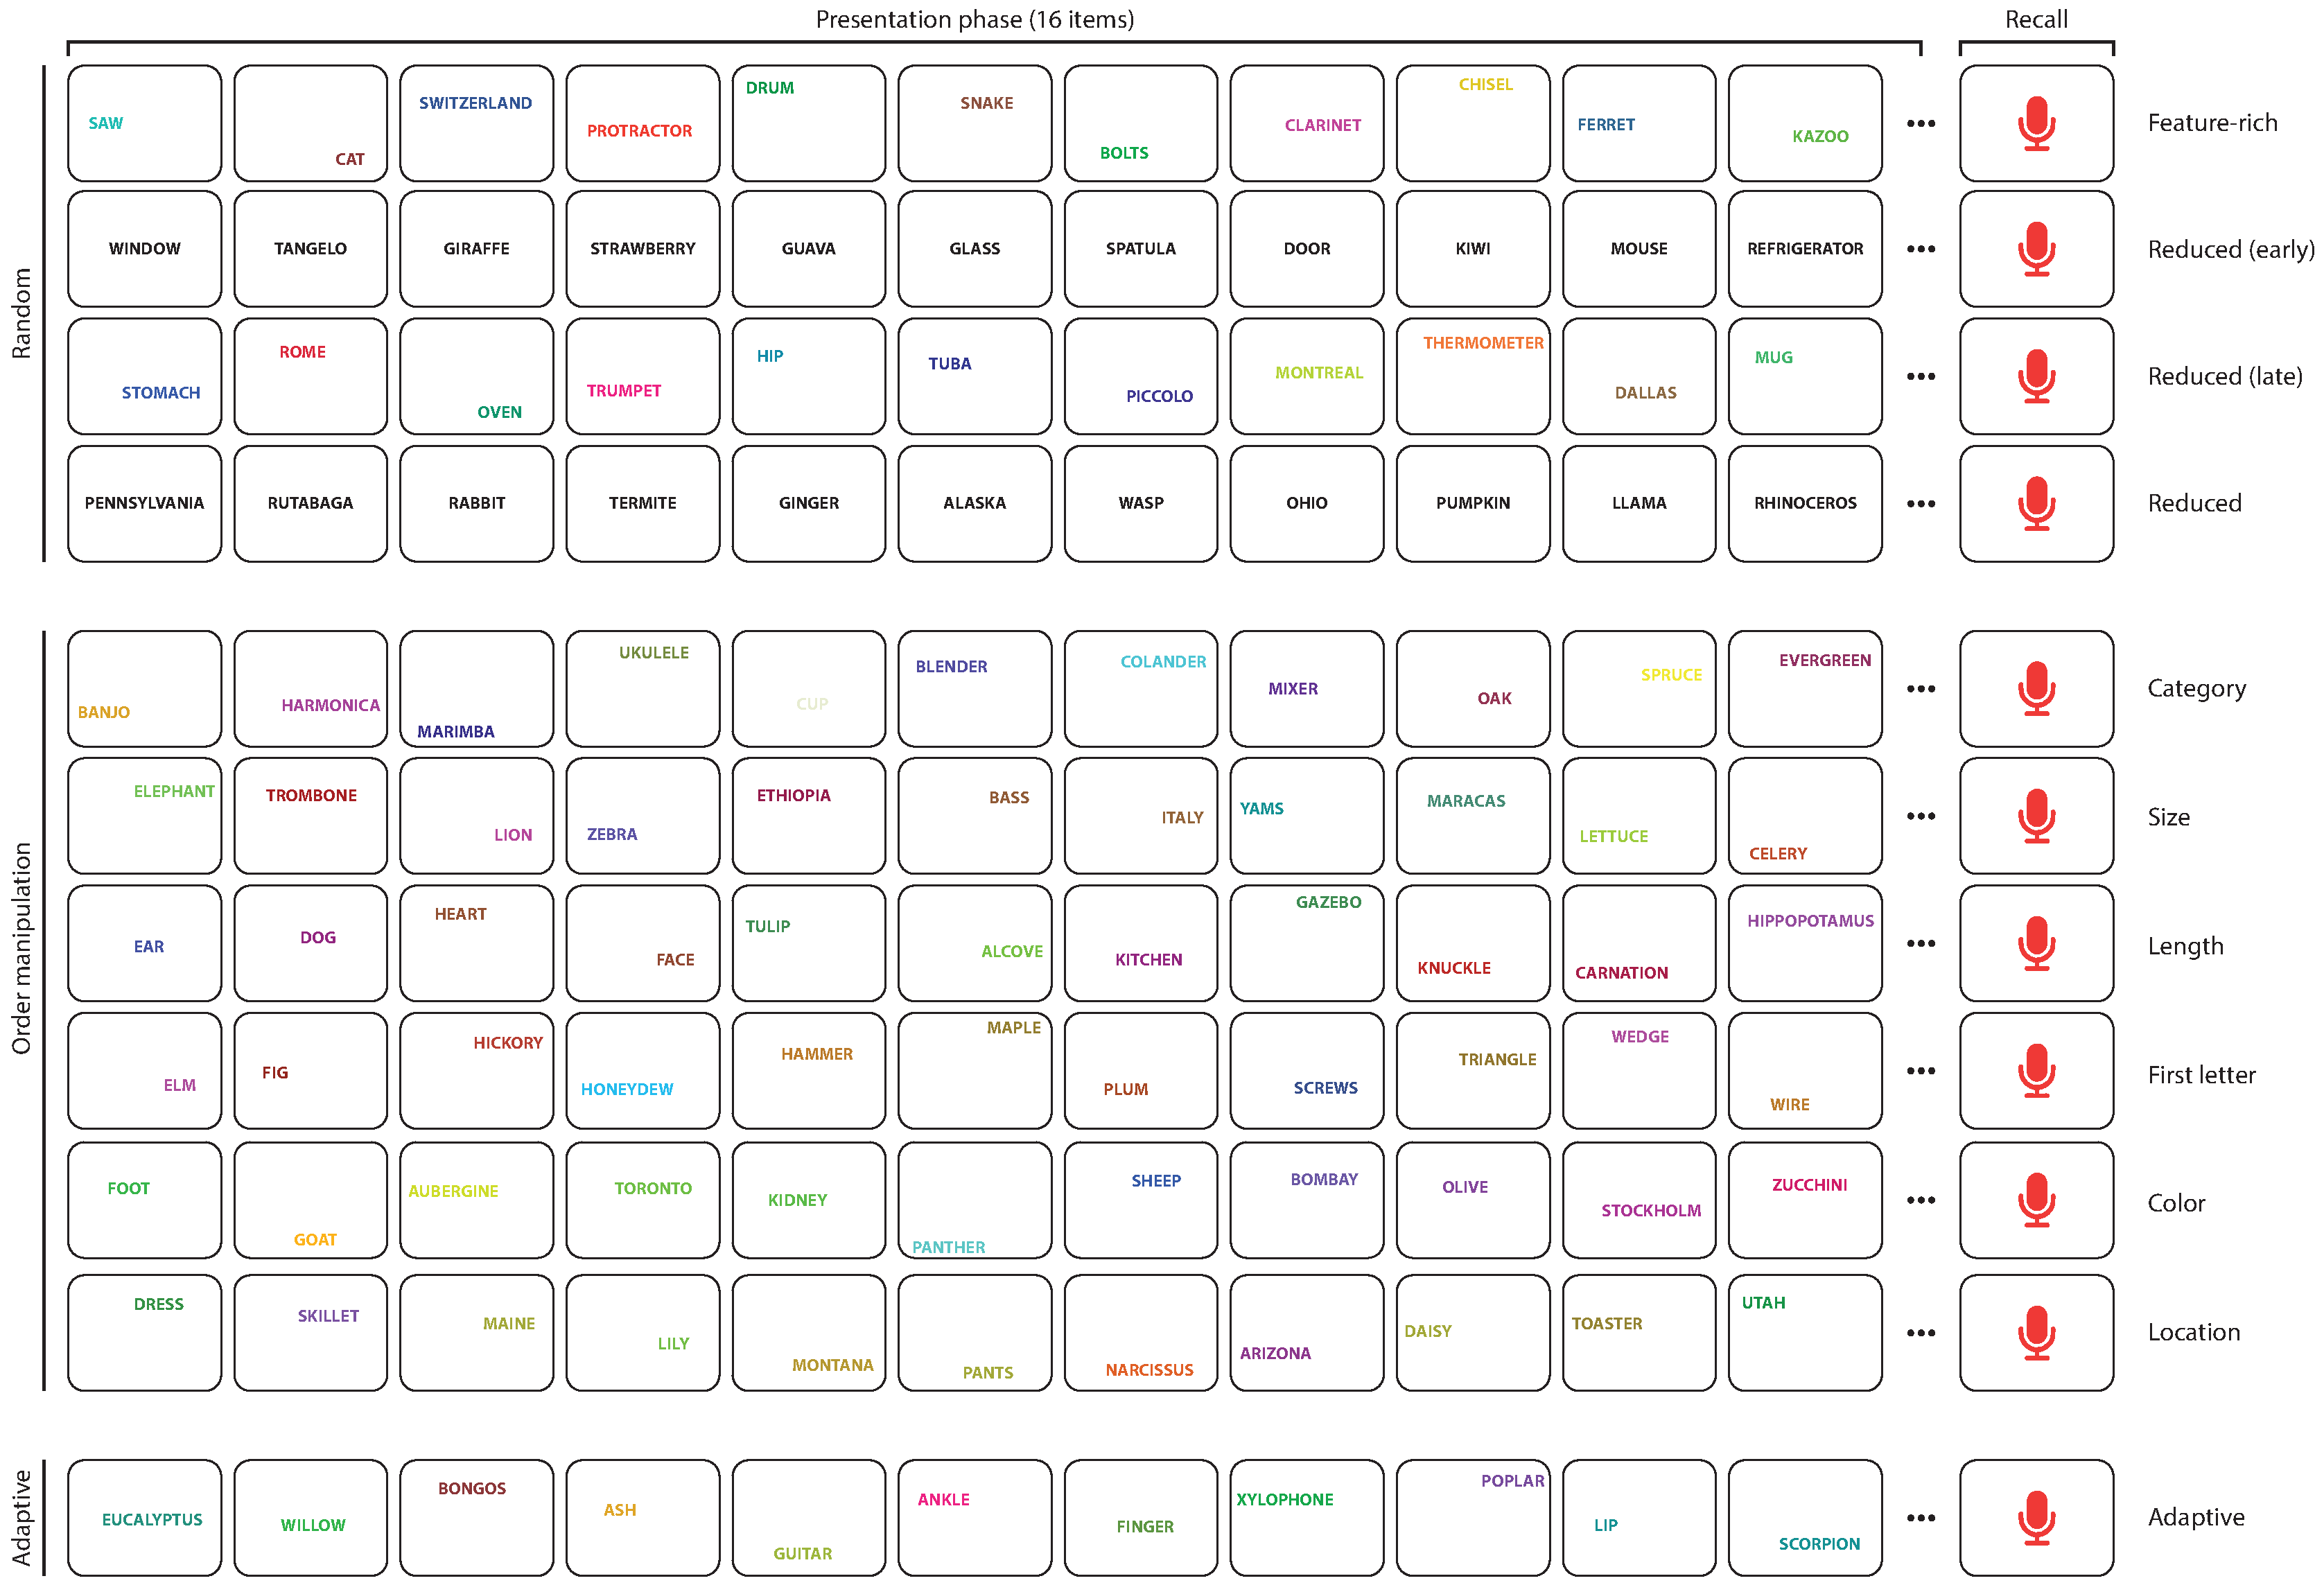
\includegraphics[width=\textwidth]{figures/FRFR}
        
\caption{\textbf{Feature-rich free recall.} After studying lists comprised of
words that vary along several feature dimensions, participants verbally recall
words in any order (microphone icon). Each experimental condition manipulates
word features and/or presentation orders within and/or across lists. The rows
display representative (illustrated) examples of items from the first list
participants might encounter in each condition. The rectangles during the
``Presentation phase'' show illustrated screen captures during a series of word
presentations. Each word appeared onscreen for 2 seconds, followed by 2 seconds
of blank screen. The red microphone icons during the ``Recall'' phase denote
the one minute verbal recall interval. The labels on the right (and
corresponding groupings on the left) denote experimental condition labels.}

    \label{fig:exp}
\end{figure}



\subsubsection*{Stimuli}

The stimuli in our paradigm were 256 English words selected in a previous
study~\citep{ZimaEtal18}. The words all referred to concrete nouns, and were
chosen from 15 unique semantic categories: body parts, building-related,
cities, clothing, countries, flowers, fruits, insects, instruments,
kitchen-related, mammals, (US) states, tools, trees, and vegetables. We also
tagged each word according to the approximate size of the object the word
referred to. Words were labeled as ``small'' if the corresponding object was
likely able to ``fit in a standard shoebox'' or ``large'' if the object was
larger than a shoebox. Most semantic categories comprised words that reflected
both ``small'' and ``large'' object sizes, but several included only one or the
other (e.g., all countries, US states, and cities are larger than a shoebox;
mean number of different sizes per category: 1.33; standard deviation: 0.49).
The numbers of words in each semantic category also varied from 12--28 (mean
number of words per category: 17.07; standard deviation number of words: 4.65).
We also identified lexicographic features for each word, including the words'
first letters and lengths (i.e., number of letters). Across all categories, all
possible first letters were represented except for `Q' (average number of
unique first letters per category: 11; standard deviation: 2 letters). Word
lengths ranged from 3--12 letters (average: 6.17 letters; standard deviation:
2.06 letters).

We assigned the categorized words into a total of 16 lists with several
constraints. First, we required that each list contained words from exactly
four unique categories, each with exactly four exemplars from each category.
Second, we required that (across all words on the list) at least one instance
of both object sizes were represented. On average, each category was
represented in 4.27 lists (standard deviation: 1.16 lists). Aside from these
two constraints, we assigned each word to a unique list. After random
assignment, each list contained words with an average of 11.13 unique starting
letters (standard deviation: 1.15 letters) and an average word length of 6.17
letters (standard deviation: 0.34 letters).

The above assignments of words to lists was performed once across all
participants, such that every participant studied the same set of 16 lists. In
every condition we randomized the study order of these lists across
participants. For participants in most conditions, on some or all of the lists,
we also randomly varied two additional visual features associated with each
word: the presentation font color, and the word's onscreen location. These
attributes were assigned independently for each word (and for every
participant). These visual features were varied for words in all lists and
conditions except for the ``reduced'' condition (all lists), the first eight
lists of the ``reduced (early)'' condition, and the last eight lists of the
``reduced (late)'' condition. In these latter cases, words were all presented
in black at the center of the experimental computer's display.

To select a random font color for each word, we drew three integers uniformly
and at random from the interval $\left[0, 255\right]$, corresponding to the red
(r), green (g), and blue (b) color channels for that word. To assign random
presentation locations to each word, we selected two floating point numbers
uniformly and at random (one for the word's horizontal $x$-coordinate and the
other for its vertical $y$-coordinate). The bounds of these coordinates were
selected to cover the entire visible area of the display without cutting off
any part of the words. The words were shown on 27-in (diagonal) Retina 5K iMac
displays (resolution: 5120 $\times$ 2880 pixels).

Most of the experimental manipulations we carried out entailed presenting or
sorting the presented words differently on the first eight lists participants
studied (which we call \textit{early} lists) versus on the final eight lists
they studied (\textit{late} lists). Since every participant studied exactly 16
lists, every list was either ``early'' or ``late'' depending on its order in
the list study sequence.


\subsubsection*{Real-time speech-to-text processing}

Our experimental paradigm incorporates the Google Cloud Speech API
speech-to-text engine~\citep{HalpEtal16} to automatically transcribe
participants' verbal recalls into text. This allows recalls to be transcribed
in real time---a distinguishing feature of the experiment; in typical verbal
recall experiments, the audio data must be parsed and transcribed manually. In
prior work, we used a similar experimental setup (equivalent to the ``reduced''
condition in the present study) to verify that the automatically transcribed
recalls were sufficiently close to human-transcribed recalls to yield reliable
data~\citep{ZimaEtal18}. This real-time speech processing component of the
paradigm plays an important role in the ``adaptive'' condition of the
experiment, as described below.

\subsubsection*{Random conditions (Fig.~\ref{fig:exp}, top four rows)}

We used two ``control'' conditions to evaluate and explore participants'
baseline behaviors. We also used performance on these control conditions to
help interpret performance in other ``manipulation'' conditions. In the first
control condition, which we call the \textit{feature rich} condition, we
randomly shuffled the presentation order (independently for each participant)
of the words on each list. In the second control condition, which we call the
\textit{reduced} condition, we randomized word presentations as in the feature
rich condition. However, rather than assigning each word a random color and
location, we instead displayed all of the words in black and at the center of
the screen.

We also designed two conditions where we varied the words' visual appearances
across lists. In the \textit{reduced (early)} condition, we followed the
``reduced'' procedure (presenting each word in black at the center of the
screen) for early lists, and followed the ``feature rich'' procedure
(presenting each word in a random color and location) for late lists. Finally,
in the \textit{reduced (late)} condition, we followed the feature rich
procedure for early lists and the reduced procedure for late lists.

\subsubsection*{Order manipulation conditions (Fig.~\ref{fig:exp}, middle six
rows)}

Each of six \textit{order manipulation} conditions used a different
feature-based sorting procedure to order words on early lists, where each
sorting procedure relied on one relevant feature dimension. All of the
irrelevant features varied freely across words on early lists, in that we did
not consider irrelevant features in ordering the early lists. However, we note
that some features were correlated---for example, some semantic categories of
words referred to objects that tended to be a particular size, which meant that
category and size were not fully independent. On late lists, the words were
always presented in a randomized order (chosen anew for each participant). In
all of the order manipulation conditions, we varied words' font colors and
onscreen locations, as in the feature rich condition.

\paragraph{Defining feature-based distances.} Sorting words according to a
given relevant feature requires first defining a distance function for
quantifying the dissimilarity between each pair of features. This function
varied according to the type of feature under consideration. Semantic features
(category and size) are \textit{categorical}. For these features, we defined a
binary distance function: two words were considered to ``match'' (i.e., have a
distance of 0) if their labels were the same (i.e., both from the same semantic
category or both of the same size). If two words' labels were different for a
given feature, we defined the words to have a distance of 1 for that feature.
Lexicographic features (length and first letter) are \textit{discrete}. For
these features we defined a discrete distance function. Specifically, we
defined the distance between two words as either the absolute difference
between their lengths, or the absolute distance between their starting letters
in the English alphabet, respectively. For example, two words that started with
the same letter would have a ``first letter'' distance of 0, and a pair of
words starting with `J' and `A' would have a first letter distance of 9.
Because words' lengths and letters' positions in the alphabet are always
integers, these discrete distances always take on integer values. Finally, the
visual features (color and location) are \textit{continuous} and
\textit{multivariate}, in that each ``feature'' is defined by multiple
(positive) real values. We defined the ``color'' and ``location'' distances
between two words as the Euclidean distances between their $(r, g, b)$ color or
$(x, y)$ location vectors, respectively. Therefore, the color and location
distance measures always take on non-negative real values (upper-bounded at
441.67 for color, or 27~in for location, reflecting the distances between the
corresponding maximally different vectors).

\paragraph{Constructing feature-sorted lists.} Given a list of words, a
relevant feature, and each word's value(s) for that feature, we developed a
stochastic algorithm for (noisily) sorting the words. The stochastic aspect of
our sorting procedure enabled us to obtain unique orderings for each
participant. First, we choose a word uniformly and at random from the set of
words on the to-be-presented list. Second, we compute the distances between the
chosen word's feature(s) and the corresponding feature(s) of all
yet-to-be-presented words. Third, we convert these distances (between the
previously presented word's feature values, $a$, and the candidate word's
feature values, $b$) to similarity scores:

\begin{equation}
 \mathrm{similarity}(a, b) = \exp\{-\tau \cdot
\mathrm{distance}(a, b)\}, \label{eqn:similarity} 
\end{equation} 
where $\tau = 1$ in our implementation. We note that increasing the value of
$\tau$ would amplify the influence of similarity on order, and decreasing the
value of $\tau$ would diminish the influence of similarity on order. Also note
that this approach requires $\tau > 0$. Finally, we computed a set of
normalized similarity values by dividing the similarities by their sum:

\begin{equation}
\mathrm{similarity}_{\mathrm{normalized}}(a, b) = \frac{\mathrm{similarity}(a,
b)}{\sum_{i=1}^n \mathrm{similarity}(a, i)}, 
\end{equation} 
where in the denominator, $i$ takes on each of the $n$ feature values of the
to-be-presented words. The resulting set of normalized similarity scores sums
to 1.

\begin{figure}[tp]
    \centering
        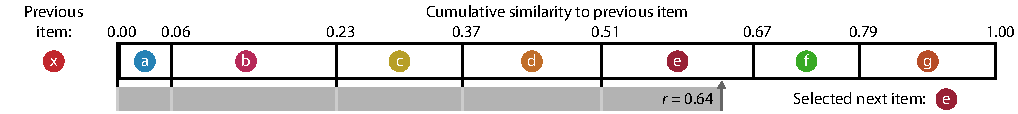
\includegraphics[width=\textwidth]{figures/stick}
        
\caption{\textbf{Generating stochastic feature-sorted lists.} For a given
feature dimension (e.g., color), we compute the similarity
(Eqn.~\ref{eqn:similarity}) between the feature value(s) of the previous item,
$x$, and all yet-to-be-presented items ($a$--$g$). Next, we normalize these
similarity scores so that they sum to 1. We lay, in sequence, a set of
``sticks,'' one for each candidate item, whose lengths are equal to these
normalized similarity scores. To select the next to-be-presented item, we draw
a random number, $r$, from the uniform distribution bounded between 0 and 1
(inclusive). The identity of the next item is given by the stick adjacent to an
indicator that moves distance $r$ (starting from 0) along the sequence of
sticks. In this case, the next to-be-presented item is $e$. Note that each
item's chances of selection is proportional to its similarity to the previous
item, along the given feature dimension (e.g., color).} \label{fig:stick}

\end{figure}

As illustrated in Figure~\ref{fig:stick}, we use these normalized similarity
scores to construct a sequence of ``sticks'' that we lay end to end in a line.
Each of the $n$ sticks corresponds to a single to-be-presented word, and the
stick lengths are proportional to the relative similarities between each word's
feature value(s) and the feature value(s) of the just-presented word. We choose
the next to-be-presented word by moving an indicator along the set of sticks,
by a distance chosen uniformly and at random on the interval $\left[0,
1\right]$. We select the word associated with the stick lying next to the
indicator to be presented next. This process continues iteratively
(re-computing the similarity scores and stochastically choosing the next
to-be-presented word using the just-presented word) until all of the words have
been presented. The result is an ordered list that tends to change gradually
along the selected feature dimension (for example ``sorted'' lists, see
Fig.~\ref{fig:exp}, \textit{Order manipulation} lists).

\subsubsection*{Adaptive condition}

We designed the \textit{adaptive} experimental condition to study the effect on
memory of lists that matched (or mismatched) the ways participants
``naturally'' organized their memories. Like the other conditions, all
participants in the adaptive condition studied a total of 16 lists, in a
randomized order. We varied the words' colors and locations for every word
presentation, as in the feature rich and order manipulation conditions.

All participants in the adaptive condition began the experiment by studying a
set of four \textit{initialization} lists. Words and features on these lists
were presented in a randomized order (computed independently for each
participant). These initialization lists were used to estimate each
participant's ``memory fingerprint,'' defined below. At a high level, a
participant's memory fingerprint describes how they prioritize or consider
different semantic, lexicographic, and/or visual features when they organize
their memories.

Next, participants studied a sequence of 12 lists in three batches of four
lists each. These batches came in three types: \textit{random},
\textit{stabilize}, and \textit{destabilize}. The batch types determined how
words on the lists in that batch were ordered. Lists in each batch were always
presented consecutively (e.g., a participant might receive four random lists,
followed by four stabilize lists, followed by four destabilize lists). The
batch orders were evenly counterbalanced across participants: there are six
possible orderings of the three batches, and 10 participants were randomly
assigned to each ordering sub-condition.

Lists in the random batches were sorted randomly (as on the initialization
lists and in the feature rich condition). Lists in the stabilize and
destabilize batches were sorted in ways that either matched or mismatched each
participant's memory fingerprint, respectively. Our procedures for estimating
participants' memory fingerprints and ordering the stabilize and destabilize
lists are described next.

\paragraph*{Feature clustering scores (uncorrected).}  

Feature clustering scores describe participants' tendencies to recall similar
presented items together in their recall sequences, where ``similarity''
considers one given feature dimension (e.g., category, color, etc.). We base
our main approach to computing clustering scores on analogous temporal and
semantic clustering scores developed by~\cite{PolyEtal09}. Computing the
clustering score for one feature dimension starts by considering the
corresponding feature values from the first word the participant recalled
correctly from the just-studied list. Next, we sort all not-yet-recalled words
in ascending order according to their feature-based distance to the
just-recalled item (see \textit{Defining feature-based distances}). We then
compute the percentile rank of the observed next recall. We average these
percentile ranks across all of the participant’s recalls for the current list
to obtain a single uncorrected clustering score for the list, for the given
feature dimension. We repeated this process for each feature dimension in turn
to obtain a single uncorrected clustering score for each list, for each feature
dimension.

\paragraph*{Temporal clustering score (uncorrected).}

Temporal clustering describes a participant's tendency to organize their recall
sequences by the learned items' encoding positions. For instance, if a
participant recalled the lists' words in the exact order they were presented
(or in exact reverse order), this would yield a score of 1. If a participant
recalled the words in a random order, this would yield an expected score of
0.5. For each recall transition (and separately for each participant), we
sorted all not-yet-recalled words according to their absolute lag (that is,
distance away in the list). We then computed the percentile rank of the next
word the participant recalled. We took an average of these percentile ranks
across all of the participant’s recalls to obtain a single (uncorrected)
temporal clustering score for the participant.


\paragraph*{Permutation-corrected feature clustering scores.}

Suppose that two lists contain unequal numbers of items of each size. For
example, suppose that list $A$ contains all ``large'' items, whereas list $B$
contains an equal mix of ``large'' and ``small'' items. For a participant
recalling list $A$, any correctly recalled item will necessarily match the size
of the previous correctly recalled item. In other words, successively recalling
several list $A$ items of the same size is essentially meaningless, since
\textit{any} correctly recalled list $A$ word will be large. In contrast,
successively recalling several list $B$ items of the same size \textit{could}
be meaningful, since (early in the recall sequence) the yet-to-be-recalled
items come from a mix of sizes. However, once all of the small items on list
$B$ have been recalled, the best possible next matching recall will be a large
item. All subsequent correct recalls must also be large items---so for
those later recalls it becomes difficult to determine whether the participant
is successively recalling large items because they are organizing their
memories according to size, or (alternatively), whether they are simply
recalling the yet-to-be-recalled items in a random order. In general, the
precise order and blend of feature values expressed in a given list, the order
and number of correct recalls a participant makes, the number of intervening
presentation positions between successive recalls, and so on, can all affect
the range of clustering scores that are possible to observe for a given list.
An uncorrected clustering score therefore conflates participants' actual memory
organization with other ``nuisance'' factors.

Following our prior work~\citep{HeusEtal17}, we used a permutation-based
correction procedure to help isolate the behavioral aspects of clustering that
we were most interested in. After computing the uncorrected clustering score
(for the given list and observed recall sequence), we compute a ``null''
distribution of $n$ additional clustering scores after randomly shuffling the
order of the recalled words (we use $n = 500$ in the present study). This null
distribution represents an approximation of the range of clustering scores one
might expect to observe by ``chance,'' given that a hypothetical participant
was \textit{not} truly clustering their recalls, but where the hypothetical
participant still studied and recalled exactly the same items (with the same
features) as the true participant. We define the \textit{permutation-corrected
clustering score} as the percentile rank of the observed uncorrected clustering
score in this estimated null distribution. In this way, a corrected score of 1
indicates that the observed score was greater than any clustering score one
might expect by chance---in other words, good evidence that the participant was
truly clustering their recalls along the given feature dimension. We applied
this correction procedure to all of the clustering scores (feature and
temporal) reported in this paper.

\paragraph*{Memory fingerprints.}

We define each participant's \textit{memory fingerprint} as the set of their
permutation-corrected clustering scores across all dimensions we tracked in our
study, including their six feature-based clustering scores (category, size,
length, first letter, color, and location) and their temporal clustering score.
Conceptually, a participant's memory fingerprint describes their tendency to
order in their recall sequences (and, presumably, organize in memory) the
studied words along each dimension. To obtain stable estimates of these
fingerprints for each participant, we averaged clustering scores across lists.
We also tracked and characterized how participants' fingerprints changed across
lists (e.g.,
Figs.~\ref{fig:fingerprint-trajectories},~\fingerprintTrajectoryRandom).

\paragraph{Online ``fingerprint'' analysis.}

The presentation orders of some lists in the adaptive condition of our
experiment (see \textit{Adaptive condition}) were sorted according to
participants' \textit{current} memory fingerprint, estimated using all of the
lists they had studied up to that point in the experiment. Because our
experiment incorporated a speech-to-text component, all of the behavioral data
for each participant could be analyzed just a few seconds after the conclusion
of the recall intervals for each list. We used the \texttt{Quail} Python
package~\citep{HeusEtal17} to apply speech-to-text algorithms to the
just-collected data, aggregate the data for the given participant, and estimate
the participant's memory fingerprint using all of their available data up to
that point in the experiment. Two aspects of our implementation are worth
noting. First, because memory fingerprints are computed independently for each
list and then averaged across lists, the already-computed memory fingerprints
for earlier lists could be cached and loaded as needed in future computations.
This meant that our computations pertaining to updating our estimate of a
participant's memory fingerprint only needed to consider data from the most
recent list. Second, each element of the null distributions of uncorrected
fingerprint scores (see \textit{Permutation-corrected feature clustering
scores}) could be estimated independently from the others. This enabled us to
make use of the testing computers' multi-core CPU architectures by considering
(in parallel) elements of the null distributions in batches of eight (i.e., the
number of CPU cores on each testing computer). Taken together, we were able to
compress the relevant computations into just a few seconds of computing time.
The combined processing time for the speech-to-text algorithm, fingerprint
computations, and permutation-based ordering procedure (described next) easily
fit within the inter-list intervals, where participants paused for a self-paced
break before moving on to study and recall the next list.

\paragraph{Ordering ``stabilize'' and ``destabilize'' lists by an estimated
fingerprint.}

In the adaptive condition of our experiment, the presentation orders for
\textit{stabilize} and \textit{destabilize} lists were chosen to either
maximally or minimally (respectively) comport with participants' memory
fingerprints. Given a participant's memory fingerprint and a to-be-presented
set of items, we designed a permutation-based procedure for ordering the items.
First, we dropped from the participant's fingerprint the temporal clustering
score. For the remaining feature dimensions, we arranged the clustering scores
in the fingerprint into a template vector, $f$. Second, we computed $n = 2500$
random permutations of the to-be-presented items. These permutations served as
candidate presentation orders. We sought to select the specific order that most
(or least) closely matched $f$. Third, for each random permutation, we computed
the (permutation-corrected) ``fingerprint,'' treating the permutation as though
it were a potential ``perfect'' recall sequence. (We did not include temporal
clustering scores in these fingerprints.) This yielded a ``simulated
fingerprint'' vector, $\hat{f}_p$ for each permutation $p$. We used these
simulated fingerprints to select a specific permutation, $i$, that either
maximized (for stabilize lists) or minimized (for destabilize lists) the
correlation between $\hat{f}_i$ and $f$.

\subsubsection*{Computing low-dimensional embeddings of memory fingerprints}

Following some of our prior work~\citep{HeusEtal18a, HeusEtal21, MannEtal22},
we use low-dimensional embeddings to help visualize how participants' memory
fingerprints change across lists
(Figs.~\ref{fig:fingerprint-trajectories}A,~\fingerprintTrajectoryRandom A). To
compute a shared embedding space across participants and experimental
conditions, we concatenated the full set of across-participant average
fingerprints (for all lists and experimental conditions) to create a large
matrix with number-of-lists (16) $\times$ number-of-conditions (10, encluding
the adaptive condition) rows and seven columns (one for each feature clustering
score, plus an additional temporal clustering score column). We used principal
components analysis to project the seven-dimensional observations into a
two-dimensional space (using the two principal components that explained the
most variance in the data). For two visualizations
(Figs.~\ref{fig:fingerprint-trajectories}B,~and~\fingerprintTrajectoryRandom B),
we computed an additional set of two-dimensional embeddings for the
\textit{average} fingerprints across lists within a given list grouping (i.e.,
early or late). For those visualizations, we averaged across the rows (for each
condition and group of lists) in the combined fingerprint matrix prior to
projecting it into the shared two-dimensional space. This yielded a single
two-dimensional coordinate for each \textit{list group} (in each condition),
rather than for each individual list. We used these embeddings solely for
visualization. All statistical tests were carried out in the original
(seven-dimensional) feature spaces.

\subsection*{Analyses}

\subsubsection*{Probability of $n$\textsuperscript{th} recall curves}

Probability of first recall curves~\citep{AtkiShif68, PostPhil65, WelcBurn24}
reflect the probability that an item will be recalled first, as a function of
its serial position during encoding. To carry out this analysis, we initialized
(for each participant) a number-of-lists (16) by number-of-words-per-list (16)
matrix of 0s. Then, for each list, we found the index of the word that was
recalled first, and we filled in that position in the matrix with a 1. Finally,
we averaged over the rows of the matrix to obtain a 1 by 16 array of
probabilities, for each participant. We used an analogous procedure to compute
probability of $n$\textsuperscript{th} recall curves for each participant.
Specifically, we filled in the corresponding matrices according to the
$n$\textsuperscript{th} recall on each list that each participant made. When a
given participant had made fewer than $n$ recalls for a given list, we simply
excluded that list from our analysis when computing that participant's
curve(s). The probability of first recall curve corresponds to a special case
where $n = 1$.

\subsubsection*{Lag-conditional response probability curve}

The lag-conditional response probability (lag-CRP) curve~\citep{Kaha96}
reflects the probability of recalling a given item after the just-recalled
item, as a function of their relative encoding positions (lag). In other words,
a lag of 1 indicates that a recalled item was presented immediately after the
previously recalled item, and a lag of $-3$ indicates that a recalled item came
three items before the previously recalled item. For each recall transition
(following the first recall), we computed the lag between the just-recalled
word's presentation position and the next-recalled word's presentation
position. We computed the proportions of transitions (between successively
recalled words) for each lag, normalizing for the total numbers of possible
transitions. In carrying out this analysis, we excluded all incorrect recalls
and successive repetitions (i.e., recalling the same word twice in a row). This
yielded, for each list, a 1 by number-of-lags ($-15$ to $+15$; 30 lags in
total, excluding lags of 0) array of conditional probabilities. We averaged
these probabilities across lists to obtain a single lag-CRP for each
participant. Because transitions at large absolute lags are rare, these curves
are typically displayed using range restrictions~\citep{Kaha12}.



\subsubsection*{Serial position curve}

Serial position curves~\citep{Murd62a} reflect the proportion of participants
who remember each item as a function of the items' serial positions during
encoding. For each participant, we initialized a number-of-lists (16) by
number-of-words-per-list (16) matrix of 0s. Then, for each correct recall, we
identified the presentation position of the word and entered a 1 into that
position (row: list; column: presentation position) in the matrix. This
resulted in a matrix whose entries indicated whether or not the words presented
at each position, on each list, were recalled by the participant (depending on
whether the corresponding entires were set to 1 or 0). Finally, we averaged
over the rows of the matrix to yield a 1 by 16 array representing the
proportion of words at each position that the participant remembered.

\subsubsection*{Identifying event boundaries}

We used the distances between feature values for successively presented words
(see \textit{Defining feature-based distances}) to estimate ``event
boundaries'' where the feature values changed more than
usual~\citep{EzzyDava11, MannEtal16,RadvCope06, SwalEtal09, SwalEtal11,
DuBrDava16}. For each list, for each feature dimension, we computed the
distribution of distances between the feature values for successively presented
words. We defined event boundaries (e.g., Fig.~\ref{fig:recall-dynamics}B) as
occurring between any successive pair of words whose distances along the given
feature dimension were greater than one standard deviation above the mean for
that list. Note that, because event boundaries are defined for each feature
dimension, each individual list may contain several sets of event boundaries,
each at different moments in the presentation sequence (depending on the
feature dimension of interest).

\section*{Results}

While holding the set of words (and the assignments of words to lists)
constant, we manipulated two aspects of participants' experiences of studying
each list. We sought to understand the effects of these manipulations on
participants' memories for the studied words. First, we added two additional
sources of visual variation to the individual word presentations: font color
and onscreen location. Importantly, these visual features were independent of
the meaning or semantic content of the words (e.g., word category, size of the
referent, etc.) and of the lexicographic properties of the words (e.g., word length,
first letter, etc.). We wondered whether this additional word-independent information
might facilitate recall (e.g., by providing new potential ways of organizing or
retrieving memories of the studied words) or impair recall (e.g., by
distracting participants with irrelevant information). Second, we manipulated
the orders in which words were studied (and how those orderings changed over
time). We wondered whether presenting the same list of words with different
appearances (e.g., by manipulating font size and onscreen location) or in
different orders (e.g., sorted along one feature dimension versus another)
might serve to influence how participants organized their memories of the
words. We also wondered whether some order manipulations might be temporally
``sticky'' by influencing how \textit{future} lists were remembered.

To obtain a clean preliminary estimate of the consequences on memory of
randomly varying the font colors and locations of presented words (versus
holding the font color fixed at black, and holding the display locations fixed
at the center of the display) we compared participants' performance on the
\textit{feature rich} and \textit{reduced} experimental conditions (see
\textit{Random conditions}, Fig.~\dynamicsRandom). In the feature rich
condition the words' colors and locations varied randomly across words, and in
the reduced condition words were always presented in black, at the center of
the display. Aggregating across all lists for each participant, we found no
difference in recall accuracy (i.e., the proportions of correctly recalled
words) for feature rich versus reduced lists ($t(126) = -0.290, p = 0.772$).
However, participants in the feature rich condition clustered their recalls
substantially more along every dimension we examined (temporal clustering:
$t(126) = 10.624, p < 0.001$; semantic category clustering: $t(126) = 10.077, p
< 0.001$; size clustering: $t(126) = 11.829, p < 0.001$; word length
clustering: $t(126) = 10.639, p < 0.001$; first letter clustering: $t(126) =
7.775, p < 0.001$; see \textit{Permutation-corrected feature clustering scores}
for more information about how we quantified each participant's clustering
tendencies.) Taken together, these comparisons suggest that adding new features
changes how participants organize their memories of studied words, even when
those new features are independent of the words themselves and even when the
new features vary randomly across words. We found no evidence that those
additional uninformative features were distracting (in terms of their impact on
memory performance), but they did affect participants' recall dynamics
(measured via their clustering scores).

We also wondered whether adding these incidental visual features to later lists
(after the participants had already studied impoverished lists), or removing
the visual features from later lists (after the participants had already
studied visually diverse lists) might affect memory performance. In other
words, we sought to test for potential effects of changing the ``richness'' of
participants' experiences over time. All participants studied and recalled a
total of 16 lists; we defined \textit{early} lists as the first eight lists and
\textit{late} lists as the last eight lists each participant encountered. To
help interpret our results, we compared participants' memories on early versus
late lists in the above feature rich and reduced conditions. Participants in
both conditions remembered more words on early versus late lists (feature rich:
$t(66) = 4.553, p < 0.001$; reduced: $t(60) = 2.434, p = 0.018$). Participants
in the feature rich (but not reduced) conditions exhibited more temporal
clustering on early versus late lists (feature rich: $t(66) = 2.318, p =
0.024$; reduced: $t(60) = 0.929, p = 0.357$). And participants in both
conditions exhibited more semantic (category and size) clustering on early
versus late lists (feature rich, category: $t(66) = 3.805, p < 0.001$; feature
rich, size: $t(66) = 2.190, p = 0.032$; reduced, category: $t(60) = 2.856, p =
0.006$; reduced, size: $t(60) = 2.947, p = 0.005$). Participants in the reduced
(but not feature rich) conditions exhibited more lexicographic clustering on
early versus late lists (feature rich, word length: $t(66) = 0.161, p = 0.872$;
feature rich, first letter: $t(66) = 0.410, p = 0.683$; reduced, word length:
$t(60) = 3.528, p = 0.001$; reduced, first letter: $t(60) = 2.275, p = 0.026$).
Taken together, these comparisons suggest that even when the presence or
absence of incidental visual features is stable across lists, participants
still exhibit some differences in their performance and memory organization
tendencies for early versus late lists.

With these differences in mind, we next compared participants' memories on
early versus late lists for two additional experimental conditions (see
\textit{Random conditions}, Fig.~\dynamicsRandom). In a \textit{reduced
(early)} condition, we held the irrelevant visual features constant on early
lists, but allowed them to vary randomly on late lists. In a \textit{reduced
(late)} condition, we allowed the irrelevant visual features to vary randomly
on early lists, but held them constant on late lists. Given our above findings
that (a) participants tended to remember more words and exhibit stronger
clustering effects on feature rich (versus reduced) lists, and (b) participants
tended to remember more words and exhibit stronger clustering effects on early
(versus late) lists, we expected these early versus late differences to be
enhanced in the reduced (early) condition and diminished in the reduced (late)
condition. However, to our surprise, participants in \textit{neither} condition
exhibited reliable early versus late differences in accuracy (reduced (early):
$t(41) = 1.499, p = 0.141$; reduced (late): $t(40) = 1.462, p = 0.152$),
temporal clustering (reduced (early): $t(41) = 0.998, p = 0.324$; reduced
(late): $t(40) = 1.099, p = 0.278$), nor feature-based clustering (reduced
(early), category: $t(41) = 0.753, p = 0.456$; reduced (early), size: $t(41) =
0.721, p = 0.475$; reduced (early), length: $t(41) = 0.493, p = 0.625$; reduced
(early), first letter: $t(41) = 0.780, p = 0.440$; reduced (late), category:
$t(40) = -0.086, p = 0.932$; reduced (late), size: $t(40) = 0.746, p = 0.460$;
reduced (late), length: $t(40) = 1.476, p = 0.148$; reduced (late), first
letter: $t(40) = 0.966, p = 0.340$). We hypothesized that adding or removing
the irrelevant features was acting as a sort of ``event boundary'' between
early and late lists. In prior work, we (and others) have found that memories
formed just after event boundaries can be enhanced~\citep[e.g., due to less
contextual interference between pre- and post-boundary items;][]{MannEtal16,
PettEtal16, GoldEtal17, FlorEtal17}.

We found that \textit{adding} irrelevant visual features on later lists that
had not been present on early lists (as in the reduced (early) condition)
served to enhance recall performance relative to conditions where all lists had
the same blends of features (accuracy for feature rich versus reduced (early):
$t(107) = -2.230, p = 0.028$; reduced versus reduced (early): $t(101) = -2.045,
p = 0.043$; also see Fig.~\accuracyByList A). However, \textit{subtracting}
irrelevant visual features on later lists that \textit{had} been present on
early lists (as in the reduced (late) condition) did not appear to impact
recall performance (accuracy for feature rich versus reduced (late): $t(106) =
-0.638, p = 0.525$; reduced versus reduced (late): $t(100) = -0.407, p =
0.685$). These comparisons suggest that recall accuracy has a directional
component: accuracy is affected differently by removing features later
that had been present earlier versus adding features later that had
\textit{not} been present earlier. In contrast, we found that participants
exhibited more temporal and feature-based clustering when we added irrelevant
visual features to \textit{any} lists (comparisons of clustering on feature
rich versus reduced lists are reported above; temporal clustering in reduced
versus reduced (early) and reduced versus reduced (late) conditions: $t$s $\leq
-9.780$, $p$s $< 0.001$; feature-based clustering in reduced versus reduced
(early) and reduced versus reduced (late) conditions: $t$s $\leq -5.443$, $p$s
$< 0.001$). Temporal and feature-based clustering were not reliably different
in the feature rich, reduced (early), and reduced (late) conditions (temporal
clustering in feature rich versus reduced (early) and feature rich versus
reduced (late) conditions: $t$s $\geq -1.434$, $p$s $\geq 0.154$; feature-based
clustering in feature rich versus reduced (early) and feature rich versus
reduced (late) conditions: $t$s $\geq -1.359$, $p$s $> 0.177$).

Taken together, our findings thus far suggest that adding item features that
change over time, even when they vary randomly and independently of the items,
can enhance participants' overall memory performance and can also enhance
temporal and feature-based clustering. To the extent that the number of item
features that vary from moment to moment approximates the ``richness'' of
participants' experiences, our findings suggest that participants remember
``richer'' stimuli better and organize richer stimuli more reliably in their
memories. Next, we turn to examine the memory effects of varying the temporal
ordering of different stimulus features while holding the features themselves
constant. We hypothesized that changing the orders in which participants were
exposed to the words on a given list might enhance (or diminish) the relative
influence of different features. For example, presenting a set of words
alphabetically might enhance participants' attention to the studied items'
first letters, whereas sorting the same list of words by semantic category
might instead enhance participants' attention to the words' semantic
attributes. Importantly, we expected these order manipulations to hold even
when the variation in the total set of features (across words) was held
constant across lists (e.g., unlike in the reduced (early) and reduced (late)
conditions, where variations in visual features were added or removed from a
subset of the lists participants studied).

\begin{figure}[tp] \centering
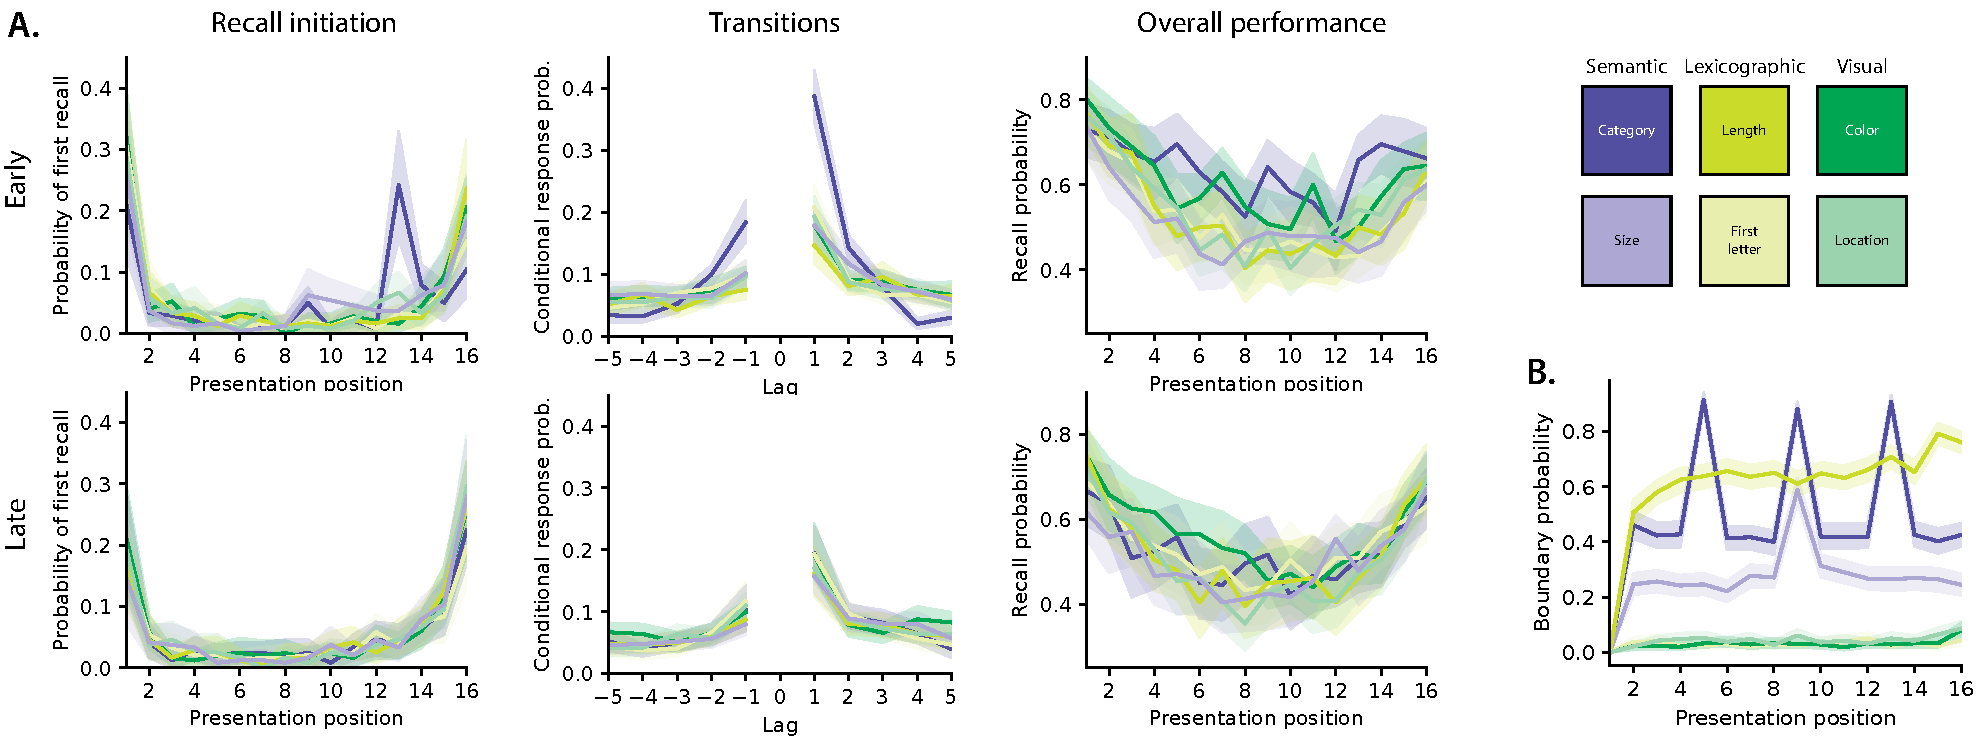
\includegraphics[width=\textwidth]{figures/recall_dynamics}

\caption{\textbf{Recall dynamics in feature rich free recall (order
manipulation conditions).} \textbf{A.} Behavioral plots. \textbf{Left panels.}
The probabilities of initiating recall with each word are plotted as a function
of presentation position. \textbf{Middle panels.} The conditional probabilities
of recalling each word are plotted as a function of the relative position (Lag)
to the words recalled just-prior. \textbf{Right panels.} The overall
probabilities of recalling each word are plotted as a function of presentation
position. \textbf{All panels.} Error ribbons denote bootstrap-estimated 95\%
confidence intervals (calculated across participants). Top panels display the
recall dynamics for early (order manipulation) lists in each condition (color).
Bottom panels display the recall dynamics for late (randomly ordered) lists.
See Figures~\dynamicsRandom~and~\dynamicsAdaptive~for analogous plots for the
random and adaptive conditions. \textbf{B.} Proportion of event boundaries (see
\textit{Identifying event boundaries}) for each condition's feature of focus,
plotted as a function of presentation position.}

    \label{fig:recall-dynamics}
\end{figure}

Across each of six order manipulation conditions, we sorted early lists by one
feature dimension but randomly ordered the items on late lists (see
\textit{Order manipulation conditions}; features: category, size, length, first
letter, color, and location). Participants in the category-ordered condition
showed an increase in memory performance on early lists (accuracy, relative to
early feature rich lists; $t(95) = 3.034, p = 0.003$). Participants in the
color-ordered condition also showed a trending increase in memory performance
on early lists (again, relative to early feature rich lists: $t(96) = 1.850, p
= 0.067$). Participants' performances on early lists in all of the other order
manipulation conditions were indistinguishable from performance on the early
feature rich lists ($\|t\|$s $< 1.013, p$s $> 0.314$). Participants in both of
the semantically ordered conditions exhibited stronger temporal clustering on
early lists (versus early feature rich lists; category: $t(95) = 8.508, p <
0.001$; size: $t(95) = 2.429, p = 0.017$). Participants in the length-ordered
condition tended to exhibit \textit{less} temporal clustering on early lists
relative to early feature rich lists ($t(95) = -1.666, p = 0.099$), whereas
participants in the first letter-ordered condition exhibited stronger temporal
clustering on early lists ($t(95) = 2.587, p = 0.011$). Participants in the
visually ordered conditions exhibited more similar performance on early lists,
relative to early feature rich lists (color: $t(96) = -1.064, p = 0.290$; we
found a trending enhancement for participants in the location-ordered
condition: $t(95) = 1.682, p = 0.096$). We also compared feature-based
clustering on early lists across the order manipulation and feature rich
conditions. Since these results were similar across both semantic conditions
(category and size), both lexicographic conditions (length and first letter),
and both visual conditions (color and location), here we aggregate data from
conditions that manipulated each of these three feature groupings in our
comparisons, to simplify the presentation. On early lists, participants in the
semantically ordered conditions exhibited stronger semantic clustering relative
to participants in the feature rich condition (category: $t(125) = 2.524, p =
0.013$; size: $t(125) = 3.510, p = 0.001$), but showed no reliable differences
in lexicographic (length: $t(125) = 0.539, p = 0.591$; first letter: $t(125) =
-0.587, p = 0.558$) or visual (color: $t(125) = -0.579, p = 0.564$; location:
$t(125) = -0.346, p = 0.730$) clustering. Similarly, participants in the
lexicographically ordered conditions exhibited stronger (relative to feature
rich participants) lexicographic clustering (length: $t(125) = 3.426, p =
0.001$; first letter: $t(125) = 3.236, p = 0.002$) on early lists, but showed
no reliable differences in semantic (category: $t(125) = -1.078, p = 0.283$;
size: $t(125) = -0.310, p = 0.757$) or visual (color: $t(125) = -0.209, p =
0.835$; location: $t(125) = -0.004, p = 0.997$) clustering. And participants in
the visually ordered conditions exhibited stronger visual clustering (again,
relative to feature rich participants, and on early lists; color: $t(126) =
2.099, p = 0.038$; location: $t(126) = 4.392, p < 0.001$), but showed no
reliable differences in semantic (category: $t(126) = 0.204, p = 0.839$; size:
$t(126) = -0.093, p = 0.926$) or lexicographic (length: $t(126) = 0.714, p =
0.476$; first letter: $t(126) = 0.820, p = 0.414$) clustering. Taken together,
these order manipulation results suggest several broad patterns
(Figs.~\ref{fig:recall-dynamics}A, \ref{fig:fingerprints}). First, most of the
order manipulations we carried out did \textit{not} reliably affect overall
recall performance. Second, most of the order manipulations increased
participants' tendencies to temporally cluster their recalls. Third, all of the
order manipulations enhanced participants' clustering of each condition's
target feature (i.e., semantic manipulations enhanced semantic clustering,
lexicographic manipulations enhanced lexicographic clustering, and visual
manipulations enhanced visual clustering) while leaving clustering along other
feature dimensions roughly unchanged (i.e., semantic manipulations did not
affect lexicographic or visual clustering, and so on).

\begin{figure}[tp] \centering
    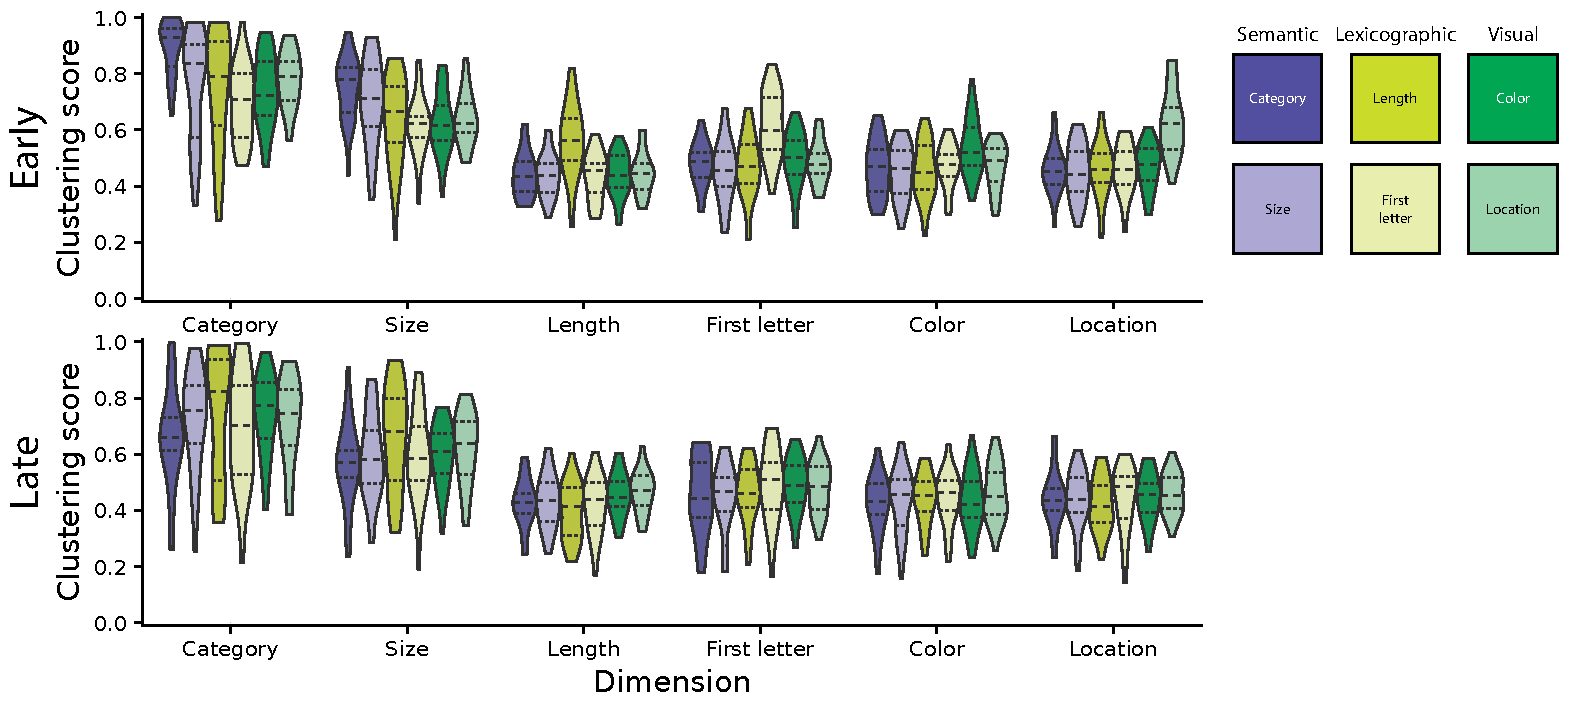
\includegraphics[width=\textwidth]{figures/fingerprints}
    
\caption{\textbf{Memory ``fingerprints'' (order manipulation conditions).} The
across-participant distributions of clustering scores for each feature type
($x$-coordinate) are displayed for each experimental condition (color),
separately for order manipulation (early, top) and randomly ordered (late,
bottom) lists. See Figures~\fingerprintsRandom~and~\fingerprintsAdaptive~for
analogous plots for the random and adaptive conditions.}
\label{fig:fingerprints}

\end{figure}

When we closely examined the sequences of words participants recalled from
early order-manipulated lists (Fig.~\ref{fig:recall-dynamics}A, top panel), we
noticed several differences from the dynamics of participants' recalls of
randomly ordered lists (Figs.~\dynamicsRandom,~\recallInit). One difference is
that participants in the category condition (dark purple curves,
Fig.~\ref{fig:recall-dynamics}) most often initiated recall with the
fourth-from-last item (\textit{Recall initiation}, top left panel), whereas
participants who recalled randomly ordered lists tended to initiate recall with
either the first or last list items (Fig.~\dynamicsRandom, top left panel). We
hypothesized that the participants might be ``clumping'' their recalls into
groups of items that shared category labels. Indeed, when we compared the
positions of feature changes in the study sequence
(Fig.~\ref{fig:recall-dynamics}B; see \textit{Identifying event boundaries})
with the positions of items participants recalled first, we noticed a striking
correspondence in both semantic conditions. Specifically, on category-ordered
lists, the category labels changed every four items on average (dark purple
peaks in Fig.~\ref{fig:recall-dynamics}B), and participants also seemed to
display an increased tendency (relative to other order manipulation and random
conditions) to initiate recall of category-ordered lists with items whose study
positions were integer multiples of four. Similarly, for size-ordered lists,
the size labels changed every eight items on average (light purple peaks in
Fig.~\ref{fig:recall-dynamics}B), and participants also seemed to display an
increased tendency to initiate recall of size-ordered lists with items whose
study positions were integer multiples of eight. A second striking difference
is that participants in the category condition exhibited a much steeper lag-CRP
(Fig.~\ref{fig:recall-dynamics}A, top middle panel) than participants in other
conditions. (This is another expression of participants' increased tendencies
to temporally cluster their recalls on category-ordered lists, as we reported
above.) Taken together, these order-specific idiosyncrasies suggest a
hierarchical set of influences on participants' memories. At longer timescales,
``event boundaries'' (to use the term loosely) can be induced across lists by
adding or removing irrelevant visual features. At shorter timescales, ``event
boundaries'' can be induced across items (within a single list) by adjusting
how item features change throughout the list.

The above comparisons between memory performance on early lists in the order
manipulation versus feature rich conditions highlight how sorted lists are
remembered differently from random lists. We also wondered how sorting lists
along each feature dimension influenced memory relative to sorting lists along
the other feature dimensions. Participants trended towards remembering early
lists that were sorted semantically better than lexicographically sorted lists
($t(118) = 1.936, p = 0.055$). Participants also remembered visually sorted
lists better than lexicographically sorted lists ($t(119) = 2.145, p = 0.034$).
However, participants showed no reliable differences in recall for semantically
versus visually sorted lists ($t(119) = 0.113, p = 0.910$). Participants
temporally clustered semantically sorted lists more strongly than either
lexicographically ($t(118) = 5.572, p < 0.001$) or visually ($t(119) = 6.215, p
< 0.001$) sorted lists, but did not show reliable differences in temporal
clustering on lexicographically versus visually sorted lists ($t(119) = 0.189,
p = 0.850$). Participants also showed reliably more semantic clustering on
semantically sorted lists than lexicographically (category: $t(118) = 3.492, p
= 0.001$, size: $t(118) = 3.972, p < 0.001$) or visually (category: $t(119) =
2.702, p = 0.008$, size: $t(119) = 4.230, p < 0.001$) sorted lists; more
lexicographic clustering on lexicographically sorted lists than semantically
(length: $t(118) = 3.112, p = 0.002$; first letter: $t(118) = 3.686, p =
0.000$) or visually (length: $t(119) = 3.024, p = 0.003$; first letter: $t(119)
= 2.644, p = 0.009$) sorted lists; and more visual clustering on visually
sorted lists than semantically (color: $t(119) = -2.659, p = 0.009$; location:
$t(119) = -4.604, p < 0.001$) or lexicographically (color: $t(119) = -2.366, p
= 0.020$; location: $t(119) = -4.265, p < 0.001$) sorted lists. In summary,
sorting lists by different features appeared to have slightly different effects
on overall memory performance and temporal clustering.  Participants also tended to
cluster their recalls along a given feature dimension more when the studied
lists were (versus were not) sorted along that dimension.

Beyond affecting how we process and remember \textit{ongoing} experiences, what
is happening to us now can also affect how we process and remember
\textit{future} experiences. Within the framework of our study, we wondered: if
early lists are sorted along different feature dimensions, might this affect
how people remember later (random) lists? In exploring this question, we
considered both group-level effects (i.e., effects that tended to be common
across individuals) and participant-level effects (i.e., effects that were
idiosyncratic across individuals).

\begin{figure}[tp] \centering
    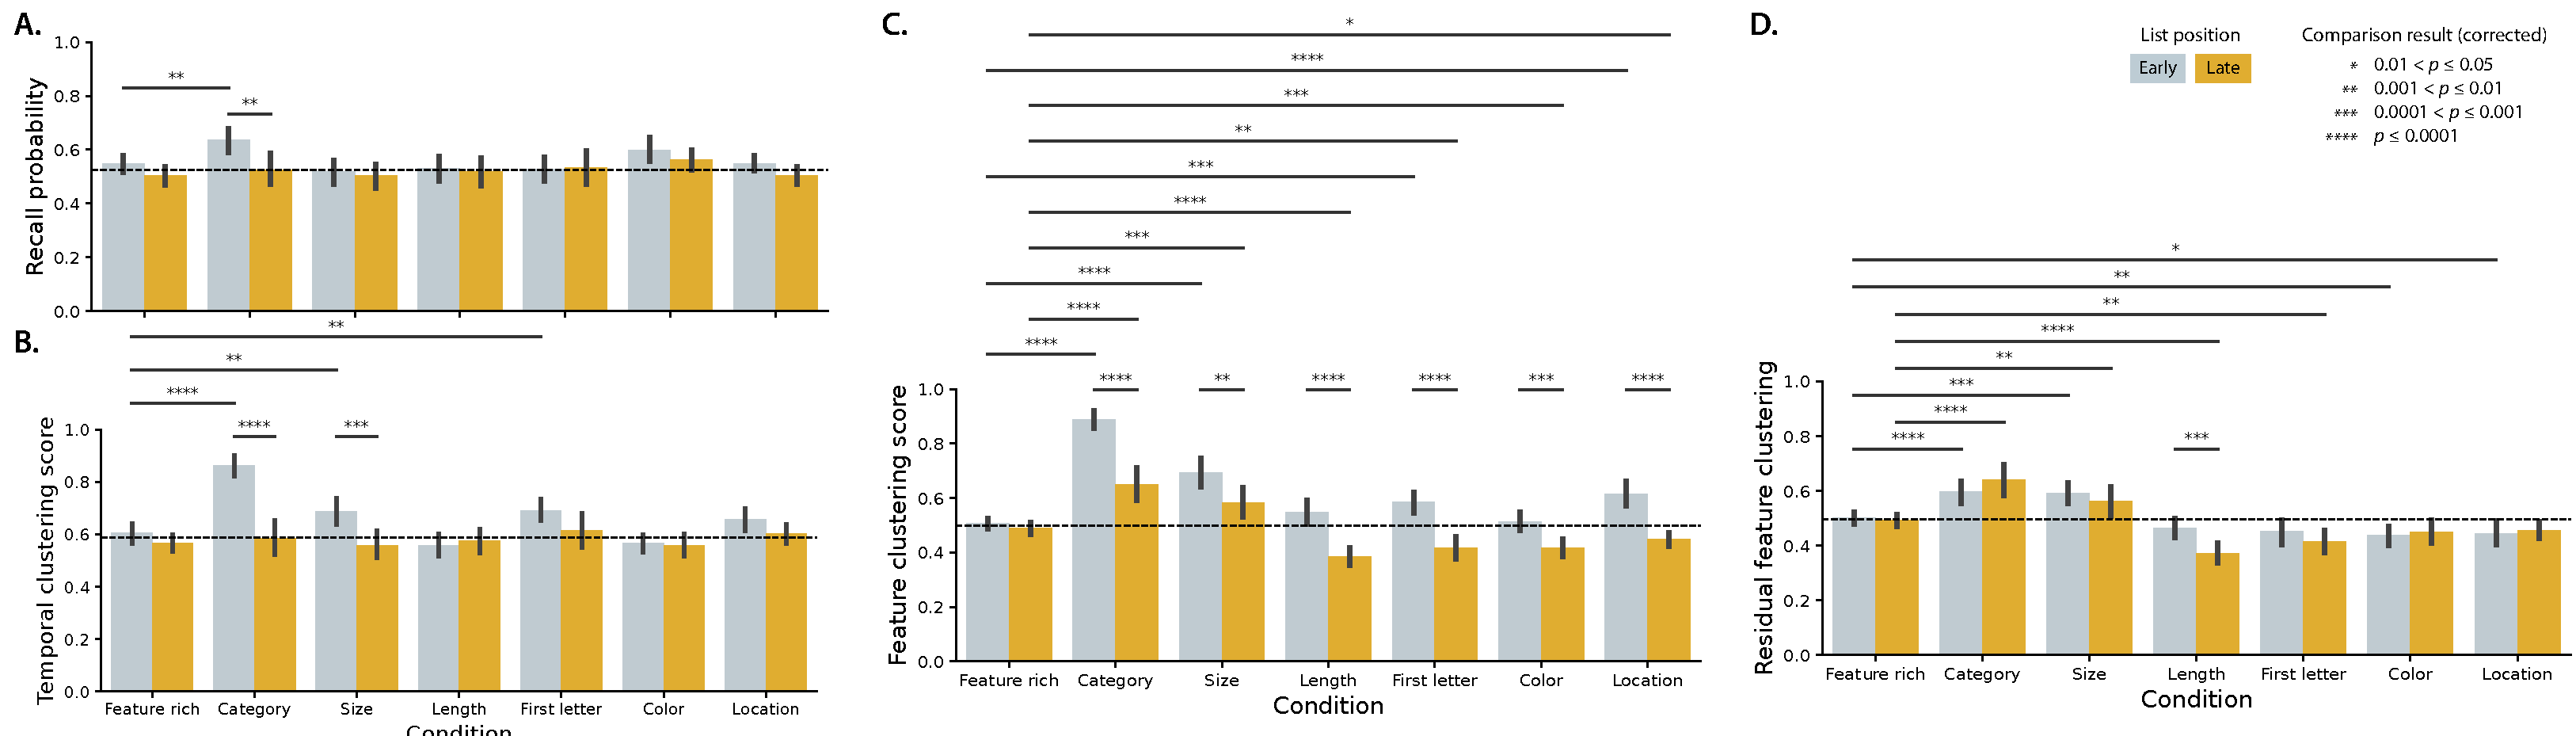
\includegraphics[width=0.7\textwidth]{figures/memory_perf_barchart_compare}
    
\caption{\textbf{Recall probability and clustering scores on early and late
lists.} The bar heights display the average (across participants) recall
probabilities (\textbf{A.}), temporal clustering scores (\textbf{B.}), and
feature clustering scores (\textbf{C.}) for early (gray) and late (gold) lists.
For the feature rich bars (left), the feature clustering scores are averaged
across features. For the order manipulation conditions, feature clustering
scores are displayed for the focused-on feature for each condition (e.g.,
category clustering scores are displayed for the category condition, and so
on). All panels: error bars denote bootstrap-estimated 95\% confidence
intervals. The horizontal dotted lines denote the average values (across all
lists and participants) for the feature rich condition.
\textbf} \label{fig:barplots}

\end{figure}

At the group level, there seemed to be almost no lingering impact of sorting
early lists on memory for later lists. To simplify the presentation, we report
these null results in aggregate across the three feature groupings. Relative to
memory performance on late feature rich lists, participants' memory performance
in all six order manipulation conditions showed no reliable differences
(semantic: $t(125) = 0.487, p = 0.627$; lexicographic: $t(125) = 0.878, p =
0.382$; visual: $t(126) = 1.437, p = 0.153$). Nor did we observe any reliable
differences in temporal clustering on late lists (relative to late feature rich
lists; semantic: $t(125) = 0.146, p = 0.884$; lexicographic: $t(125) = 0.923, p
= 0.358$; visual: $t(126) = 0.525, p = 0.601$). Aside from a slightly increased
tendency for participants to cluster words by their length on late visual order
manipulation lists (more than late feature rich lists; $t(126) = 2.199, p =
0.030$), we observed no reliable differences in any type of feature clustering
on late order manipulation condition lists versus late feature rich lists
($\|t\|$s $\leq 1.234, p$s $\geq 0.220$).

We also looked for more subtle group-level patterns. For example, perhaps
sorting early lists by one feature dimension could affect how participants
cluster \textit{other} features (on early and/or late lists) as well. We
defined participants' \textit{memory fingerprints} as the set of their temporal
and feature clustering scores (see \textit{Memory fingerprints}). A
participant's memory fingerprint describes how they tend to retrieve memories
of the studied items, perhaps searching through several feature spaces (or
along several representational dimensions). To gain insights into the dynamics
of how participants' clustering scores tended to change over time, we computed
the average (across participants) fingerprint from each list, from each order
manipulation condition (Fig.~\ref{fig:fingerprint-trajectories}). We projected
these fingerprints into a two-dimensional space to help visualize the dynamics
(top panels; see \textit{Computing low-dimensional embeddings of memory
fingerprints}). We found that participants' average fingerprints tended to
remain relatively stable on early lists, and exhibited a ``jump'' to another
stable state on later lists. The sizes of these jumps varied somewhat across
conditions (the Euclidean distances between fingerprints in their original high
dimensional spaces are displayed in the bottom panels). We also averaged the
fingerprints across early and late lists, respectively, for each condition
(Fig.~\ref{fig:fingerprint-trajectories}B). We found that participants'
fingerprints on early lists seem to be influenced by the order manipulations
for those lists (see the locations of the circles in
Fig.~\ref{fig:fingerprint-trajectories}B). There also seemed to be some
consistency across different features within a broader type. For example, both
semantic feature conditions (category and size; purple markers) diverge in a
similar direction from the group; both lexicographic feature conditions (length
and first letter; yellow markers) diverge in a similar direction; and both
visual conditions (color and location; green) also diverge in a similar
direction. But on late lists, participants' fingerprints seem to return to a
common state that is roughly shared across conditions (i.e., the stars in that
panel are clumped together).

\begin{figure}[tp] \centering
    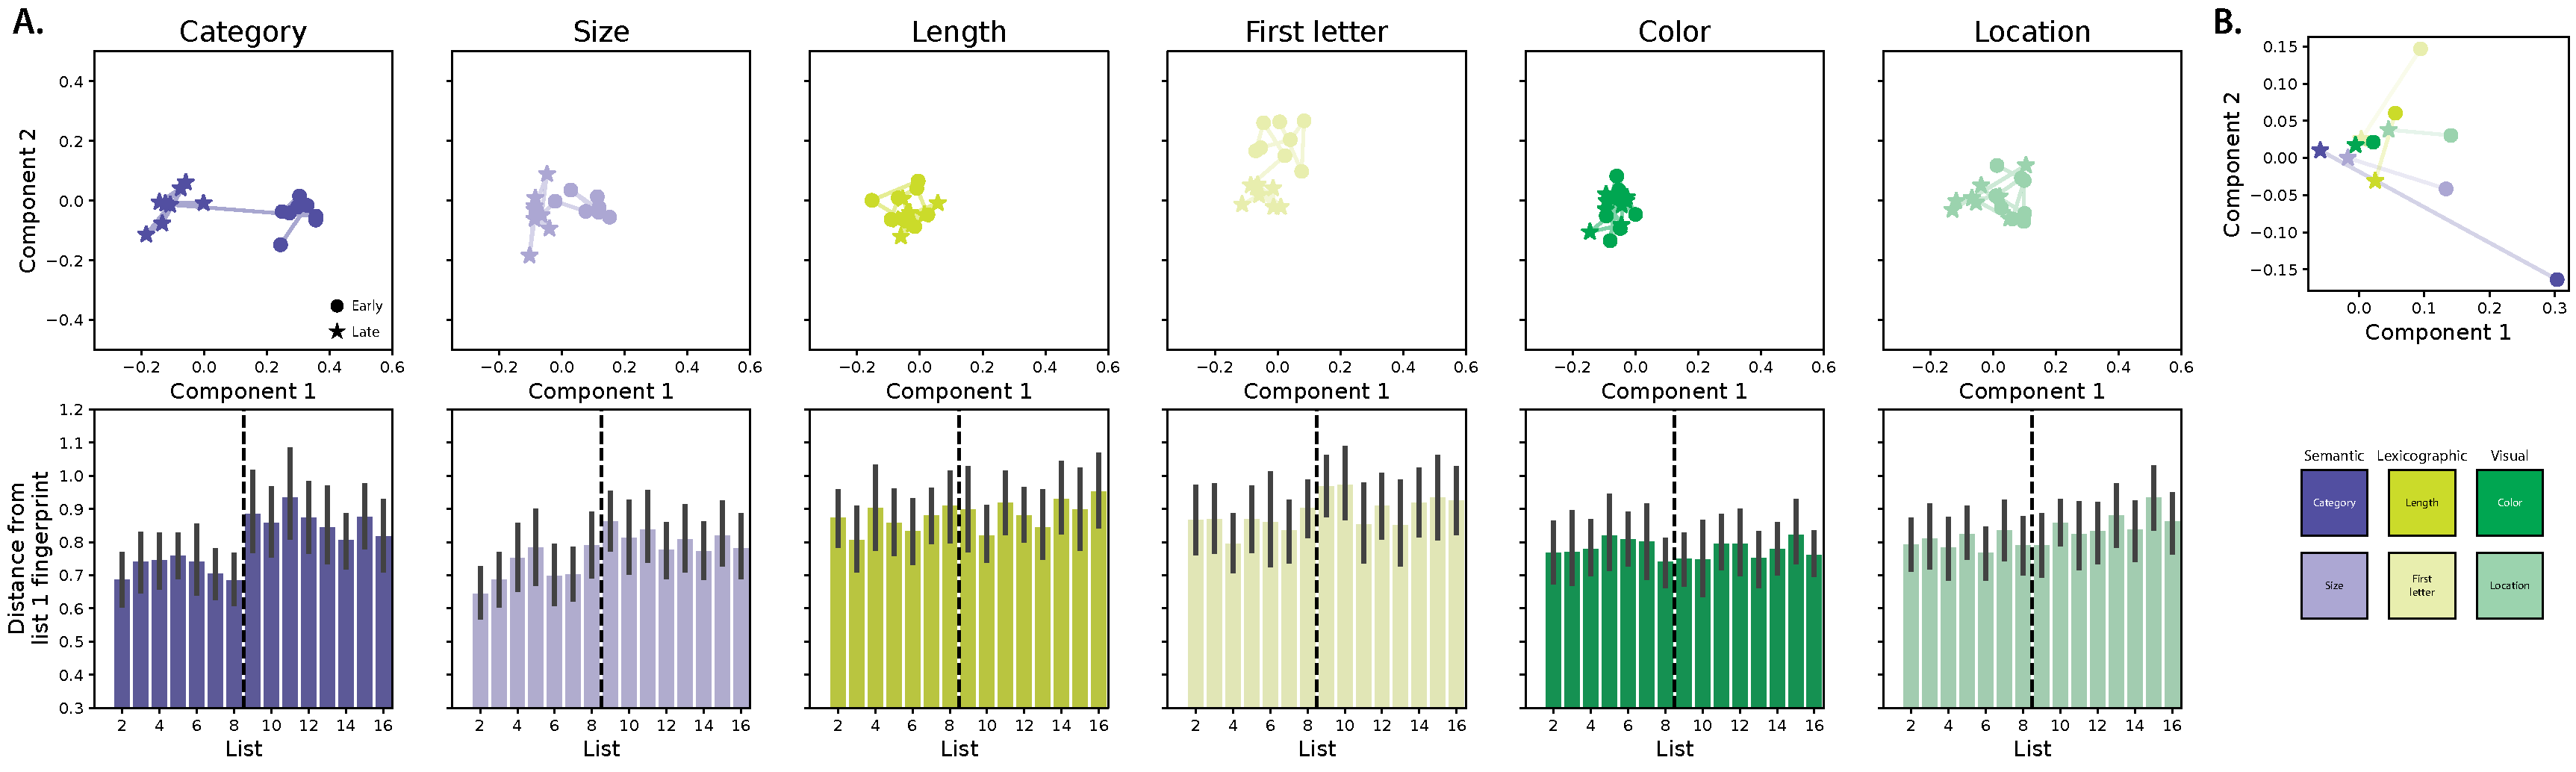
\includegraphics[width=\textwidth]{figures/fingerprint_trajectories}
    
    \caption{\textbf{Memory fingerprint dynamics (order manipulation
    conditions).} \textbf{A.} Each column (and color) reflects an experimental
    condition. In the top panels, each marker displays a 2D projection of the
    (across-participant) average memory fingerprint for one list. Order
    manipulation (early) lists are denoted by circles and randomly ordered
    (late) lists are denoted by stars. All of the fingerprints (across all
    conditions and lists) are projected into a common space. The bar plots in
    the bottom panels display the Euclidean distances of the per-list memory
    fingerprints to the list 0 fingerprint, for each condition. Error bars
    denote bootstrap-estimated 95\% confidence intervals. The dotted vertical
    lines denote the boundaries between early and late lists. \textbf{B.} In
    this panel, the fingerprints for early (circle) and late (star) lists are
    averaged across lists and participants before projecting the fingerprints
    into a (new) 2D space. See Figure~\fingerprintTrajectoryRandom~for
    analogous plots for the random conditions. }
    \label{fig:fingerprint-trajectories}
    
    \end{figure}

When we examined the data at the level of individual participants
(Figs.~\ref{fig:clustering-scatterplots} and \ref{fig:clustering-carryover}), a
clearer story emerged. Within each order manipulation condition, participants
exhibited a range of feature clustering scores on both early and late lists
(Fig.~\ref{fig:clustering-scatterplots}A, B). Across every order manipulation
condition, participants who exhibited stronger feature clustering (for their
condition's manipulated feature) recalled more words. This trend held overall
across conditions and participants (early: $r(179) = 0.537, p < 0.001$; late: $
r(179) = 0.492, p < 0.001$) as well as for each condition individually for
early ($r$s $\geq 0.386$, all $p$s $\leq 0.035$) and late ($r$s $\geq 0.462$,
all $p$s $\leq 0.010$) lists. We found no evidence of a condition-level trend;
for example, the conditions where participants tended to show stronger
clustering scores were not correlated with the conditions where participants
remembered more words (early: $r(4) = 0.526, p = 0.284$; late: $r(4) = -0.257,
p = 0.623$; see insets of Fig.~\ref{fig:clustering-scatterplots}A and B). We
observed carryover associations between feature clustering and recall
performance (Fig.~\ref{fig:clustering-scatterplots}C, D). Participants who
showed stronger feature clustering on early lists tended to recall more items
on late lists (across conditions: $r(179) = 0.492, p < 0.001$; all conditions
individually: $r$s $\geq 0.462$, all $p$s $\leq 0.010$). Participants who
recalled more items on early lists also tended to show stronger feature
clustering on late lists (across conditions: $r(179) = 0.280, p < 0.001$; all
non-visual conditions: $r$s $\geq 0.445$, all $p$s $\leq 0.014$; color: $r(29)
= 0.298, p = 0.103$; location: $r(28) = 0.354, p = 0.055$). Neither of these
effects showed condition-level trends (early feature clustering versus late
recall probability: $r(4) = -0.299, p = 0.565$; early recall probability versus
late feature clustering: $r(4) = 0.400, p = 0.432$). We also looked for
associations between feature clustering and temporal clustering. Across every
order manipulation condition, participants who exhibited stronger feature
clustering also exhibited stronger temporal clustering. For early lists
(Fig.~\ref{fig:clustering-scatterplots}E), this trend held overall ($r(179) =
0.924, p < 0.001$), for each condition individually (all $r$s $\geq 0.822$, all
$p$s $< 0.001$), and across conditions ($r(4) = 0.964, p = 0.002$). For late
lists (Fig.~\ref{fig:clustering-scatterplots}F), the results were more variable
(overall: $r(179) = 0.348, p < 0.001$; all non-visual conditions: $r$s $\geq
0.382$, all $p$s $\leq 0.037$; color: $r(29) = 0.453, p = 0.011$; location: $
r(28) = 0.190, p = 0.314$; across-conditions: $r(4) = -0.036, p = 0.945$).
While less robust than the carryover associations between feature clustering
and recall performance, we also observed some carryover associations between
feature clustering and temporal clustering
(Fig.~\ref{fig:clustering-scatterplots}G, H). Participants who showed stronger
feature clustering on early lists trended towards showing stronger temporal
clustering on later lists (overall: $r(179) = 0.301, p < 0.001$; for individual
conditions: all $r$s $\geq 0.297$, all $p$s $\leq 0.111$; across conditions: $
r(4) = 0.107, p = 0.840$). And participants who showed stronger temporal
clustering on early lists trended towards showing stronger feature clustering
on later lists (overall: $r(179) = 0.579, p < 0.001$; all non-visual
conditions: $r$s $\geq 0.323$, all $p$s $\leq 0.082$; visual conditions: $r$s
$\geq 0.089$, all $p$s $\leq 0.632$; across conditions: $r(4) = 0.916, p =
0.010$). Taken together, the results displayed in
Figure~\ref{fig:clustering-scatterplots} show that participants who were more
sensitive to the order manipulations (i.e., participants who showed stronger
feature clustering for their condition's feature on early lists) remembered
more words and showed stronger temporal clustering. These associations also
appeared to carry over across lists, even when the items on later lists were
presented in a random order.

\begin{figure}[tp] \centering
    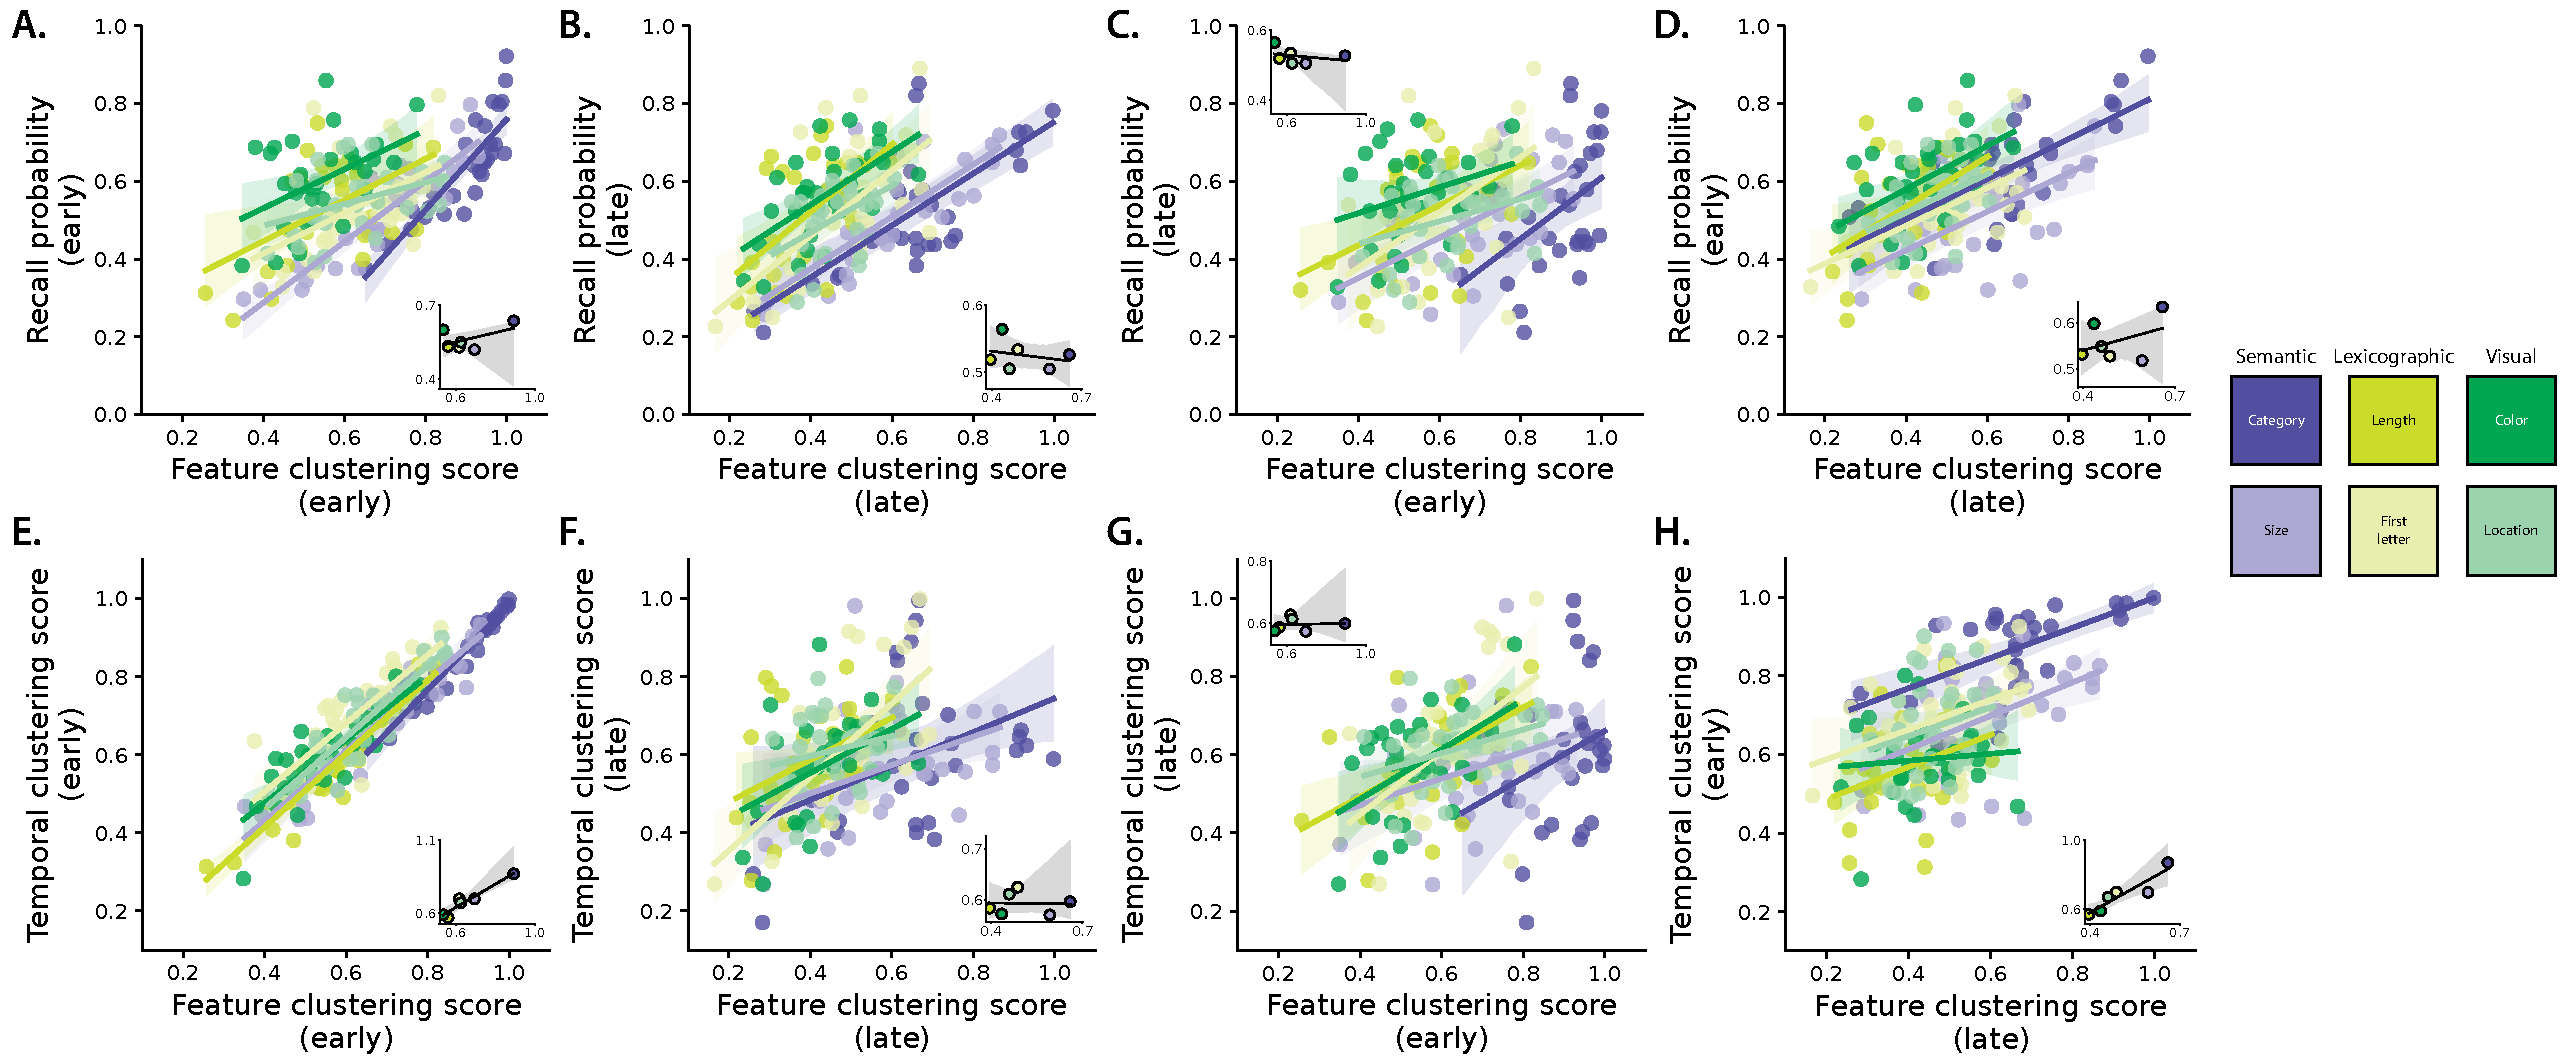
\includegraphics[width=\textwidth]{figures/feature_clustering_vs_accuracy_and_contiguity}
    
    \caption{\textbf{Interactions between feature clustering, recall probability,
    and contiguity.} \textbf{A.} Recall probability versus feature clustering
    scores for order manipulation (early) lists. \textbf{B.} Recall probability
    versus feature clustering for randomly ordered (late) lists. \textbf{C.} Recall
    probability on late lists versus feature clustering on early lists. \textbf{D.}
    Recall probability on early lists versus feature clustering on late lists.
    \textbf{E.} Temporal clustering scores (contiguity) versus feature clustering
    scores on early lists. \textbf{F.} Temporal clustering scores versus feature
    clustering scores on late lists. \textbf{G.} Temporal clustering scores on late
    lists versus feature clustering scores on early lists. \textbf{H.} Temporal
    clustering scores on early lists versus feature clustering scores on late
    lists. \textbf{All panels.} Each dot in the main scatterplots denotes the
    average scores for one participant. The colored regression lines are computed
    across participants. The inset displays condition-averaged results, where each
    dot reflects a single condition and the regression line is computed across
    experimental conditions. All error ribbons denote bootstrap-estimated 95\%
    confidence intervals.} \label{fig:clustering-scatterplots} 
    
\end{figure}

If participants show different sensitivities to order manipulations, how do
their behaviors carry over to later lists? We found that participants who
showed strong feature clustering on early lists often tended to show strong
feature clustering on late lists (Fig.~\ref{fig:clustering-carryover}A; overall
across participants and conditions: $r(179) = 0.592, p < 0.001$; non-visual
feature conditions: all $r$s $\geq 0.350$, all $p$s $\leq 0.058$; color: $r(29)
= -0.071, p = 0.704$; location: $r(28) = 0.032, p = 0.868$; across conditions:
$r(4) = 0.934, p = 0.006$). Although participants tended to show weaker feature
clustering on late lists (Fig.~\ref{fig:fingerprint-trajectories}) on
\textit{average}, the associations between early and late lists for individual
participants suggests that some influence of early order manipulations may
linger on late lists. We found that participants who exhibited larger carryover
in feature clustering (i.e., continued to show strong feature clustering on
late lists) for the semantic order manipulations (but not other manipulations)
also tended to show a larger improvement in recall
(Fig.~\ref{fig:clustering-carryover}B; overall: $r(179) = 0.378, p < 0.001$;
category: $r(28) = 0.419, p = 0.021$; size: $r(28) = 0.737, p < 0.001$;
non-semantic conditions: all $r$s $\leq 0.252$, all $p$s $\geq 0.179$; across
conditions: $r(4) = 0.773, p = 0.072$) on late lists, relative to early lists.
Participants who exhibited larger carryover in feature clustering also tended
to show stronger temporal clustering on late lists (relative to early lists)
for all but the category condition (Fig.~\ref{fig:clustering-carryover}C;
overall: $r(179) = 0.434, p < 0.001$; category: $r(28) = 0.229, p = 0.223$; all
non-category conditions: all $r$s $\geq 0.448$, all $p$s $\leq 0.012$; across
conditions: $r(4) = 0.598, p = 0.210$).

\begin{figure}[tp] \centering
    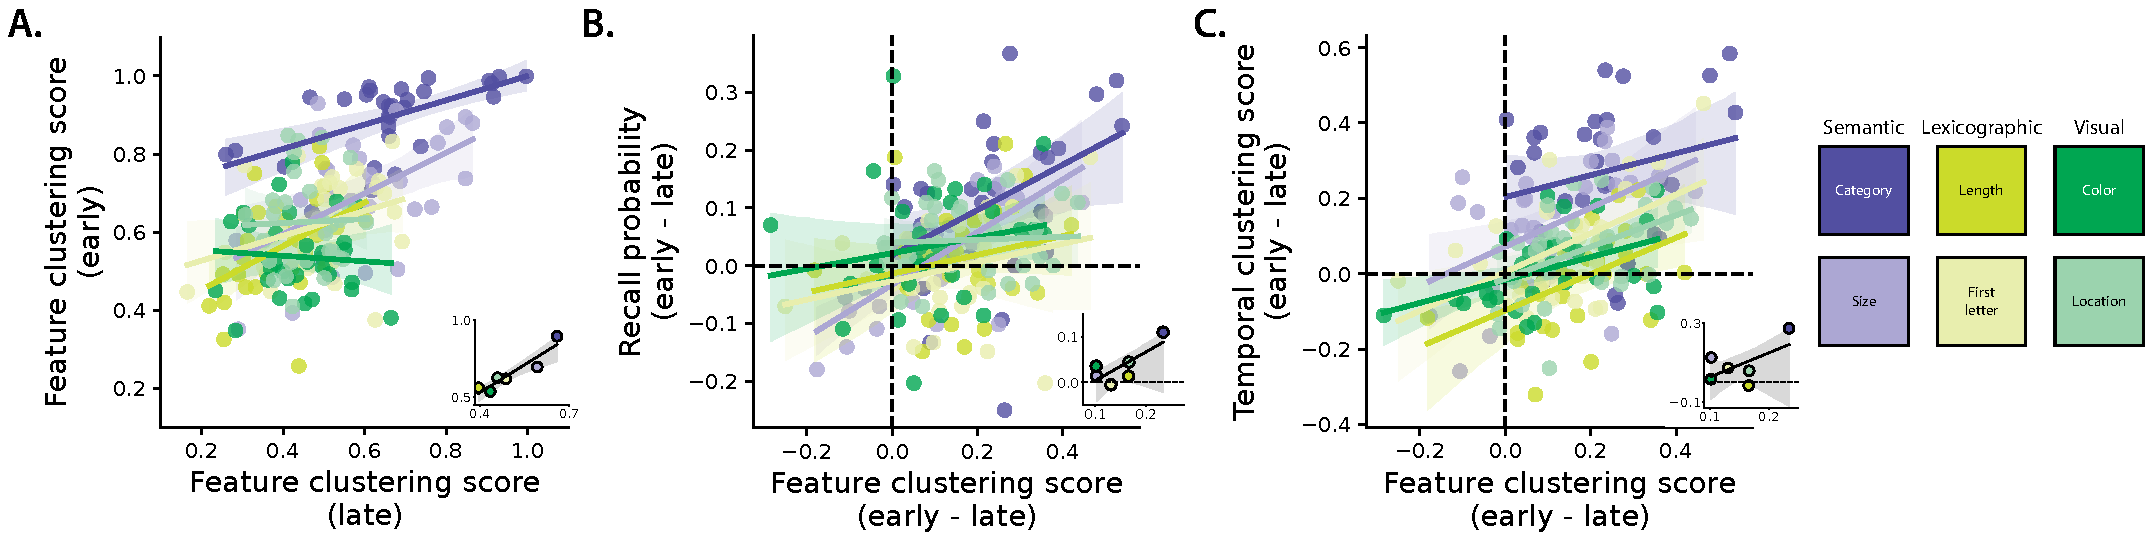
\includegraphics[width=\textwidth]{figures/clustering_carryover}
    
    \caption{\textbf{Feature clustering carryover effects.} \textbf{A.} Feature
    clustering scores for order manipulation (early) versus randomly ordered
    (late) lists. \textbf{B.} Accuracy differences (on early versus late lists)
    versus feature clustering ``carryover'' (defined as the differences between
    the average clustering scores on early and late lists). \textbf{C.}
    Temporal clustering differences (on early versus late lists) versus feature
    clustering carryover. \textbf{All panels.} Each dot in the main
    scatterplots denotes the average scores for one participant. The colored
    regression lines are computed across participants. The inset displays
    condition-averaged results, where each dot reflects a single condition and
    the regression line is computed across experimental conditions. All error
    ribbons denote bootstrap-estimated 95\% confidence intervals.}
    \label{fig:clustering-carryover} 

\end{figure}

We suggest two potential interpretations of these findings. First, it is
possible that some participants are more ``malleable'' or ``adaptable'' with
respect to how they organize incoming information. When presented with list of
items sorted along \textit{any} feature dimension, they will simply adopt that
feature as a dominant dimension for organizing those items and subsequent
(randomly ordered) items. This flexibility in memory organization might afford
such participants a memory advantage, explaining their strong recall
performance. An alternative interpretation is that each participant comes into
our study with a ``preferred'' way of organizing incoming information. If they
happen to be assigned to an order manipulation condition that matches their
preferences, then they will appear to be ``sensitive'' to the order
manipulation and also exhibit a high degree of carryover in feature clustering
from early to late lists. These participants might demonstrate strong recall
performance not because of their inherently superior memory abilities, but
rather because the specific condition they were assigned to happened to be
especially easy for them, given their pre-experimental tendencies. To help
distinguish between these interpretations, we designed an \textit{adaptive}
experimental condition (see \textit{Adaptive condition}). The primary
manipulation in the adaptive condition is that participants each experience
three key types of lists. On \textit{random} lists, words are ordered randomly
(as in the feature rich condition). On \textit{stabilize} lists, the
presentation order is adjusted to be maximally similar to the current estimate
of the participant's memory fingerprint (see \textit{Online “fingerprint”
analysis}). Third, on \textit{destabilize} lists, the presentation order is
adjusted to be \textit{minimally} similar to the current estimate of the
participant's memory fingerprint (see \textit{Ordering ``stabilize'' and
``destabilize'' lists by an estimated fingerprint}). The orders in which
participants experienced each type of list were counterbalanced across
participants to help reduce the influence of potential list-order effects.
Because the presentation orders on stabilize and destabilize lists are adjusted
to best match each participant's (potentially unique) memory fingerprint, the
adaptive condition removes uncertainty about whether participants' assigned
conditions might just ``happen'' to match their preferred ways of organizing
their memories.

\begin{figure} 
    \centering

    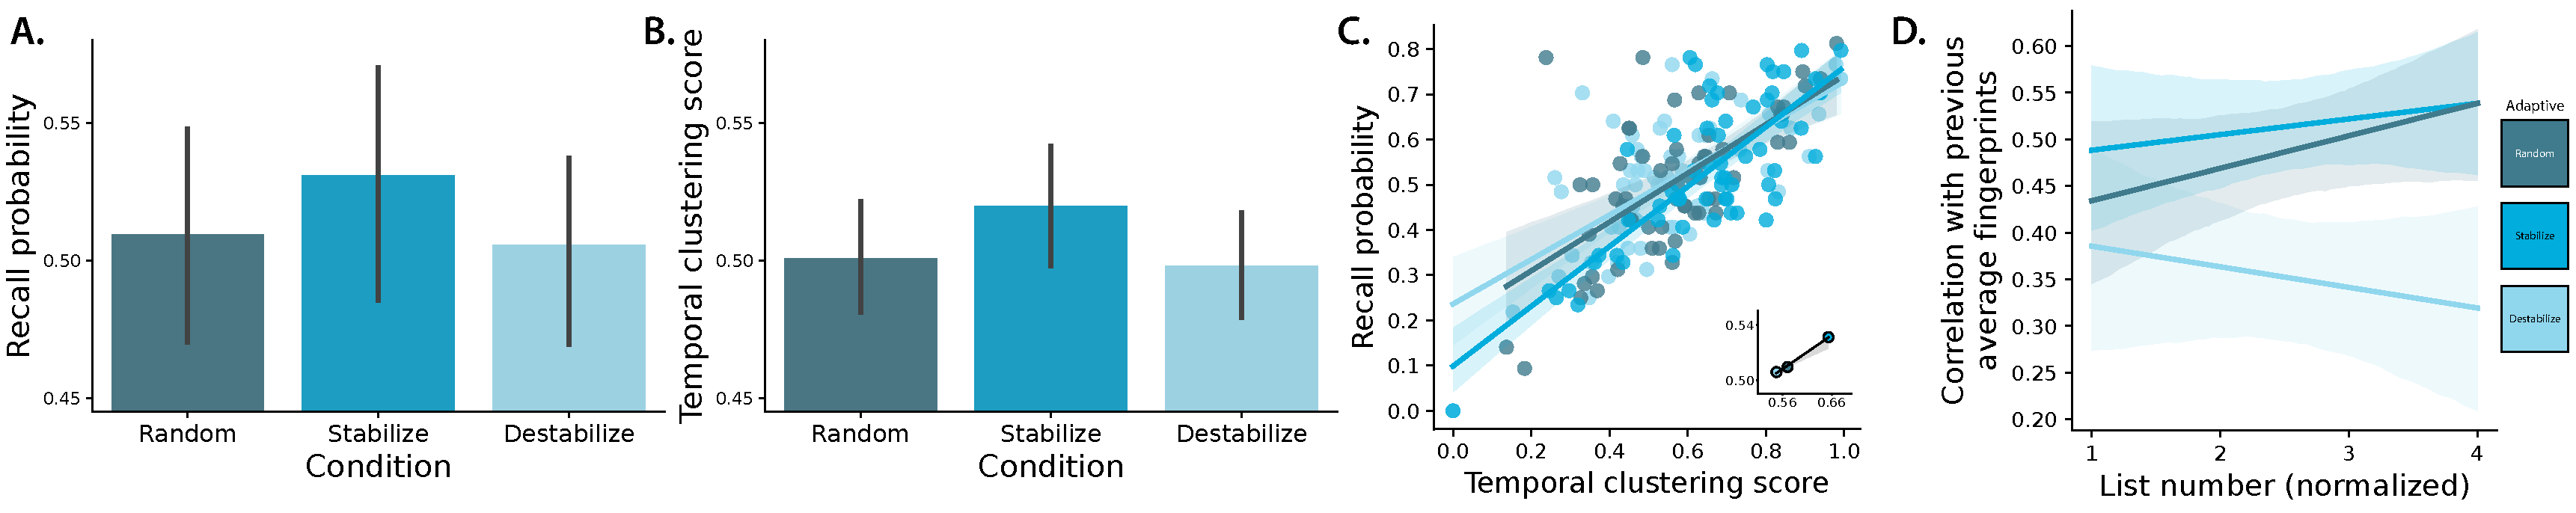
\includegraphics[width=\textwidth]{figures/adaptive_results}
        
        \caption{\textbf{Adaptive free recall.} \textbf{A.} Average probability
        of recall (taken across words, lists, and participants) for lists from
        each adaptive condition. \textbf{B.} Average temporal clustering scores
        for lists from each adaptive condition. \textbf{C.} Recall probability
        versus temporal clustering scores by participant (main panel; each
        participant contributes one dot per condition) and averaged within
        condition (inset; each dot represents a single condition). \textbf{D.}
        Per-list correlations between the current list's fingerprint and the
        average fingerprint computed from all previous lists. The normalized
        list numbers ($x$-axis) denote the number of lists of the same type
        that the participant had experienced at the time of the current list.
        All panels: Colors denote the sorting type (condition) for each list.
        Error bars and ribbons denote bootstrap-estimated 95\% confidence
        intervals. For additional details about participants' behavior and
        performance during the adaptive conditions, see
        Figure~\dynamicsAdaptive.}

    \label{fig:adaptive}
\end{figure}

Participants' fingerprints on stabilize and random lists tended to become
(numerically) slightly more similar to their average fingerprints computed from
the previous lists they had experienced, and their fingerprints on destabilize
lists tended to become numerically less similar (Fig.~\ref{fig:adaptive}D).
Overall, we found that participants tended to be better at remembering words on
stabilize lists relative to words on both random ($t(59) = 1.740, p = 0.087$)
and destabilize ($t(59) = 1.714, p = 0.092$) lists (Fig.~\ref{fig:adaptive}A).
Participants showed no reliable differences in their memory performance on
destabilize versus random lists ($t(59) = -0.249, p = 0.804$). Participants
also exhibited stronger temporal clustering on stabilize lists, relative to
random ($t(59) = 3.554, p = 0.001$) and destabilize ($t(59) = 4.045, p <
0.001$) lists (Fig.~\ref{fig:adaptive}B). We found no reliable differences in
temporal clustering for items on random versus destabilize lists ($t(59) =
-0.781, p = 0.438$).

As in the other experimental manipulations, participants in the adaptive
condition exhibited substantial variability with respect to their overall
memory performance and their clustering tendencies (Fig.~\ref{fig:adaptive}C).
We found that individual participants who exhibited strong temporal clustering
scores also tended to recall more items. This held across subjects, aggregating
across all list types ($r(178) = 0.721, p < 0.001$), and for each list type
individually (all $r$s $\geq 0.683$, all $p$s $\leq 0.001$). Taken together,
the results from the adaptive condition suggest that each participant comes
into the experiment with their own unique memory organization tendencies, as
characterized by their memory fingerprint. When participants study lists whose
items come pre-sorted according to their unique preferences, they tend to remember
more and show stronger temporal clustering.

\section*{Discussion}

% recap

We asked participants to study and freely recall word lists. The words on each
list (and the total set of lists) were held constant across participants. For
each word, we considered (and manipulated) two semantic features (category and
size) that reflected aspects of the \textit{meanings} of the words, along with
two lexicographic features (word length and first letter), which reflected
characteristics of the words' \textit{letters}. These semantic and
lexicographic features are intrinsic to each word. We also considered and
manipulated two additional visual features (color and location) that affected
the \textit{appearance} of each studied item, but could be varied independently
of the words' identities. Across different experimental conditions, we
manipulated how the visual features varied across words (within each list),
along with the orders of each list's words. Although the participants' task
(verbally recalling as many words as possible, in any order, within one minute)
remained constant across all of these conditions, and although the set of words
they studied from each list remained constant, our manipulations substantially
affected participants' memories. The impact of some of the manipulations also
affected how participants remembered \textit{future} lists that were sorted
randomly.

% specific findings:
%   reduced (early/late) vs. feature rich and reduced: event boundaries
%   order manipulations: lingering effects
%   adaptive condition: people have unique preferences, and matching them can improve their memory and affect how the remembered info is organized

\subsection*{Recap: visual feature manipulations}

We found that participants in our feature rich condition (where we varied
words' appearances) recalled similar proportions of words to participants in a
reduced condition (where appearance was held constant across words). However,
varying the words' appearances led participants to exhibit much more temporal
and feature-based clustering. This suggests that even seemingly irrelevant
elements of our experiences can affect how we remember them.

When we held the within-list variability in participants' visual experiences
fixed across lists (in the feature rich and reduced conditions), they
remembered more words from early lists than from late lists. For feature rich
lists, they also showed stronger clustering for early versus late lists.
However, when we \textit{varied} participants' visual experiences across lists
(in the ``reduced (early)'' and ``reduced (late)'' conditions), these early
versus late accuracy and clustering differences disappeared. Abruptly changing
how irrelevant visual features varied across words seemed to act as a sort of
``event boundary'' that partially reset how participants processed and
remembered post-boundary lists. Within-list clustering also increased in these
manipulations, suggesting that the ``within-event'' words were being more tightly
associated with each other.

When we held the visual features constant during early lists, but then varied
words' appearances in later lists (i.e., the reduced (early) condition),
participants' overall memory performance improved. However, this impact was
directional: when we \textit{removed} visual features from words in late lists
that had been present in early lists (i.e., the reduced (late) condition), we
saw no memory improvement.

\subsection*{Recap: order manipulations}

When we (stochastically) sorted early lists along different feature dimensions,
we found several impacts on participants' memories. Sorting early lists
semantically (by word category) enhanced participants' memories for those
lists, but the effects on performance of sorting along other feature dimensions
were inconclusive. However, each order manipulation substantially affected how
participants \textit{organized} their memories of words from the ordered lists.
When we sorted lists semantically, participants displayed stronger semantic
clustering; when we sorted lists lexicographically, they displayed stronger
lexicographic clustering; and when we sorted lists visually, they displayed
stronger visual clustering. Clustering along the unmanipulated feature
dimensions in each of these cases was unchanged.

The order manipulations we examined also appeared to induce, in some cases, a
tendency to ``clump'' similar words within a list. This was most apparent on
semantically ordered lists, where the probability of initiating recall with a
given word seemed to follow groupings defined by feature change points.

We also examined the impact of early list order manipulations on memory for
late lists. At the group level, we found little evidence for lingering
``carryover'' effects of these manipulations: participants in the order
manipulation conditions showed similar memory performance and clustering on
late lists to participants in the corresponding control (feature rich)
condition. At the level of individual participants, however, we found several
meaningful patterns.

Participants who showed stronger feature clustering on early
(order-manipulated) lists tended to better remember late (randomly ordered)
lists. Participants who remembered early lists better also tended to show
stronger feature clustering (along their condition's feature dimension) on late
lists (even though the words on those late lists were presented in a random
order). We also observed some (weaker) carryover effects of temporal
clustering. Participants who showed stronger feature clustering (along their
condition's feature dimension) on early lists tended to show stronger temporal
clustering on late lists. And participants who showed stronger temporal
clustering on early lists also tended to show stronger feature clustering on
late lists. Essentially, these order manipulations appeared to affect each
participant differently. Some participants were sensitive to our manipulations,
and those participants' memory performance was impacted more strongly, both for
the ordered lists and for future (random) lists. Other participants appeared
relatively insensitive to our manipulations, and those participants showed
little carryover effects on late lists.

These results at the individual participant level suggested to us that either
(a) some participants were more sensitive to \textit{any} order manipulation,
or (b) some participants might be more (or less) sensitive to manipulations
along \textit{particular} (e.g., preferred) feature dimensions. To help
distinguish between these possibilities, we designed an adaptive condition
whereby we attempted to manipulate whether participants studied words in an
order that either matched or mismatched our estimate of how they would cluster
or organize the studied words in memory (i.e., their idiosyncratic memory
fingerprint). We found that when we presented words in orders that were
consistent with participants' memory fingerprints, they remembered more words
overall and showed stronger temporal clustering. This comports well with the
second possibility described above. Specifically, each participant seems to
bring into the experiment their own idiosyncratic preferences and strategies
for organizing the words in their memory. When we presented the words in an
order consistent with each participant's idiosyncratic fingerprint, their
memory performance improved. This might indicate that the participants were
spending less cognitive effort ``reorganizing'' the incoming words on those
lists, which freed up resources to devote to encoding processes instead.

% connections to prior work: 
%     - context effects: role of irrelevant features, temporal context and order effects
%     - priming: being "primed" to 
%     - situation models: 

\subsection*{Context effects on memory performance and organization}

In real-world experience, each moment's unique blend of contextual features
(where we are, who we are with, what else we are thinking of at the time, what
else we experience nearby in time, etc.) plays an important role in how we
interpret, experience, and remember that moment, and how we relate it to our
other experiences~\citep[e.g., for review see ][]{Mann20}. What are the
analogues of real-world contexts in laboratory tasks like the free recall
paradigm employed in our study? In general, modern formal accounts of free
recall~\citep{Kaha20} describe context as comprising a mix of (a) features
pertaining to or associated with each item and (b) other items and thoughts
experienced nearby in time, e.g., that might still be ``lingering'' in the
participant's thoughts at the time they study the item. Item features can
include semantic properties (i.e., features related to the item's meaning),
lexicographic properties (i.e., features related to the item's letters),
sensory properties (i.e., feature related to the item's appearance, sound,
smell, etc.), emotional properties (i.e., features related to how meaningful the
item is, whether the item evokes positive or negative feelings, etc.),
utility-related properties (e.g., features that describe how an item might be
used or incorporated into a particular task or situation), and more.
Essentially any aspect of the participant's experience that can be
characterized, measured, or otherwise described can be considered to influence
the participant's mental context at the moment they experience that item.
Temporally proximal features include aspects of the participant's internal or
external experience that are \textit{not} specifically occurring at the moment
they encounter an item, but that nonetheless influence how they process the
item. Thoughts related to percepts, goals, expectations, other experiences, and
so on that might have been cued (directly or indirectly) by the participant's
recent experiences prior to the current moment all fall into this category.
Internally driven mental states, such as thinking about an experience unrelated
to the experiment, also fall into this category.

Contextual features need not be intentionally or consciously perceived by the
participant to affect memory, nor do they need to be relevant to the task
instructions or the participant's goals. Incidental factors such as font
color~\citep{JonePyc14}, background color~\citep{IsarIsar07}, inter-stimulus
images~\citep{GersEtal13, MannEtal16, ChiuEtal21}, background
sounds~\citep{BeamJone10, SahaSmit14}, secondary tasks~\citep{MasiSaha14,
PolyEtal09, OberLewa08}, and more can all impact how participants remember, and
organize in memory, lists of studied items.

Consistent with this prior work, we found that participants were sensitive to
task-irrelevant visual features. We also found that changing the dynamics of
those task-irrelevant visual features (in the reduced (early) and reduced
(late) conditions) \textit{also} affected participants' memories. This suggests
that it is not only the contextual features themselves that affect memory, but
also the \textit{dynamics} of context---i.e., how the contextual features
associated with each item change over time.

\subsection*{Priming effects on memory performance and organization}

% explicit priming (resolve ambiguous stimuli, e.g., green eyes study)
% negative priming: suppressing previously irrelevant stimuli or features hurts participants' recall for those stimuli when they're used on subsequent lists
% implicit priming (most like here): patterns in prior experiences sets expectations about what is to come, which can affect memory for upcoming stimuli
%    - participants in the reduced ({early, late}) conditions picked up on irrelevant features in early lists and when those features changed their memories for subsequent lists were affected.
%    - participants in the order manipulation conditions picked up on structure in temporal order on early lists, and that affected how they remembered later lists

When our ongoing experiences are ambiguous, we can draw on our past
experiences, expectations, and other real, perceived, or inferred cues to help
resolve these ambiguities. We may also be overtly or covertly ``primed'' to
influence how we are likely to resolve ambiguities. For example, before
listening to a story with several equally plausible interpretations, providing
participants with ``background'' information beforehand can lead them towards
one interpretation versus another~\citep{YeshEtal17}. More broadly, our
conscious and unconscious biases and preferences can influence not only how we
interpret high-level ambiguities, but even how we process low-level sensory
information~\citep{KataEtal23}.

In more simplified scenarios, like list-learning paradigms, the stimuli and
tasks participants encounter before studying a given list can influence what
and how they remember. For example, when participants are directed to suppress,
disregard, or ignore ``distracting'' stimuli early on in an experiment,
participants often tend to remember those stimuli less well when they are
re-used as to-be-remembered targets later on in the experiment~\citep{Tipp85}.
In general, participants' memories can be influenced by exposing them to a wide
range of positive and negative priming factors before they encounter the
to-be-remembered information~\citep{BaloEtal92, ClayChat89, Donn88, FlexTulv82,
GottEtal12, HuanEtal04, Hube08, HubeEtal01, McNa94, Neel77, Rabi86, TulvScha91,
WatkEtal92, WiggMart98}.

The order manipulation conditions in our experiment show that participants can
also be primed to pick up on more subtle statistical structure in their
experiences, like the dynamics of how the presentation orders of stimuli vary
along particular feature dimensions. These order manipulations affected not
only how participants remembered the manipulated lists, but also how they
remembered \textit{future} lists with different (randomized) temporal
properties.

\subsection*{Expectation, event boundaries, and situation models}

Our findings that participants' current and future memory behaviors are
sensitive to manipulations in which features change over time, and how features
change across items and lists, suggest parallels with studies on how we form
expectations and predictions, segment our continuous experiences into discrete
events, and make sense of different scenarios and situations. Each of these
real-world cognitive phenomena entail identifying statistical regularities in
our experiences, and exploiting those regularities to gain insight, form
inferences, organize or interpret memories, and so on. Our past experiences
enable us to predict what is likely to happen in the future, given what
happened ``next'' in our previous experiences that were similar to
now~\citep{Mann20, EichFort09, BarrEtal20, Brig12, ChowEtal16, GlucEtal02,
GoldEtal21, GrifStey03, JonePash07, KimEtal14, TamiThor18, XuEtal23}.

When our expectations are violated, such as when our observations disagree with
our predictions, we may perceive the ``rules'' or ``situation'' to have
changed. \textit{Event boundaries} denote abrupt changes in the state of our
experience, for example, when we transition from one situation to
another~\citep{RadvZack17, ZwaaRadv98}. Crossing an event boundary can impair
our memory for pre-boundary information and enhance our memory for
post-boundary information~\citep{RadvCope06, SahaKell02, MannEtal16,
DuBrDava13}. Event boundaries are also tightly associated with the notion of
\textit{situation models} and \textit{schemas}---mental frameworks for
organizing our understanding about the rules of how we and others are likely to
behave, how events are likely to unfold over time, how different elements are
likely to interact, and so on. For example, a situation model pertaining to a
particular restaurant might set our expectations about what we are likely to
experience when we visit that restaurant (e.g., what the building will look
like, how it will smell when we enter, how crowded the restaurant is likely to
be, the sounds we are likely to hear, etc.). Similarly, as mentioned in the
\textit{Introduction}, we might learn a schema describing how events are likely
to unfold \textit{across} any sit-down restaurant---e.g., open the door, wait
to be seated, receive a menu, decide what to order, place the order, and so on.
Situation models and schemas can help us to generalize across our experiences,
and to generate expectations about how new experiences are likely to unfold.
When those expectations are violated, we can perceive ourselves to have crossed
into a new situation.

In our study, we found that abruptly changing the ``rules'' about how the
visual appearances of words are determined, or about the orders in which words
are presented, can lead participants to behave similarly to what one might
expect upon crossing an event boundary. Adding variability in font color and
presentation location for words on late lists, after those visual features had
been held constant on early lists, led participants to remember more words on
those later lists. One potential explanation is that participants perceive an
``event boundary'' to have occurred when they encounter the first ``late''
list. According to contextual change accounts of memory across event
boundaries~\citep[e.g.,][]{SahaKell02, PettEtal16, GoldEtal17, FlorEtal17},
this could help to explain why participants in the reduced (early) and reduced
(late) conditions exhibited better overall memory performance. Specifically,
their memory for late list items could benefit from less interference from
early list items, and the contextual features associated with late list items
(after the ``event boundary'') might serve as more specific recall cues for
those late items (relative to if the boundary had not occurred).

% implications for:
%     - theory: flexibility in how we organize information, bridge between "classic" and naturalistic experiments
%     - applications: adaptive learning, education and training

\subsection*{Theoretical implications}

Although most modern formal theories of episodic memory have been developed and
tested to explain memory for list-learning tasks~\citep{Kaha20}, a number of
recent studies suggest some substantial differences between memory for lists
versus naturalistic stimuli~\citep[e.g., real-world experiences, narratives,
films, etc.;][]{NastEtal20, HeusEtal21, Mann21a, LeeEtal20}. One reason is that
naturalistic stimuli are often much more engaging than the highly simplified
list-learning tasks typically employed in the psychological laboratory, perhaps
leading participants to pay more attention, exert more effort, and stay more
consistently motivated to perform well~\citep{NastEtal20}. Another reason is
that the temporal unfoldings of events and occurrences in naturalistic stimuli
tend to be much more meaningful than the temporal unfoldings of items on
typical lists used in laboratory memory tasks. Real-world events exhibit
important associations at a broad range of timescales. For example, an early
detail in a detective story may prove to be a clue to solving the mystery later
on. Further, what happens in one moment typically carries some predictive
information about what came before or after~\citep{XuEtal23}. In contrast, the
lists used in laboratory memory tasks are most often ordered randomly, by
design, to \textit{remove} meaningful temporal structure in the
stimulus~\citep{Kaha12}.

On one hand, naturalistic stimuli provide a potential means of understanding
how our memory systems function in the circumstances we most often encounter in
our everyday lives. This implies that, to understand how memory works in the
``real world,'' we should study memory for stimuli that reflect the relevant
statistical structure of real-world experiences. On the other hand,
naturalistic stimuli can be difficult to precisely characterize or model,
making it difficult to distinguish whether specific behavioral trends follow
from fundamental workings of our memory systems, from some aspect of the
stimulus, or from idiosyncratic interactions or interference between
participants' memory systems and the stimulus. This challenge implies that, to
understand the fundamental nature of memory in its ``pure'' form, we should
study memory for highly simplified stimuli that can provide relatively unbiased
(compared with real-world experiences) measures of the relevant patterns and
tendencies.

The experiment we report in this paper was designed to help bridge some of this
gap between naturalistic tasks and more traditional list-learning tasks. We had
people study word lists similar to those used in classic memory studies, but we
also systematically varied the lists' ``richness'' (by adding or removing
visual features) and temporal structure (through order manipulations that
varied over time and across experimental conditions). We found that
participants' memory behaviors were sensitive to these manipulations. Some of
the manipulations led to changes that were common across people (e.g., more
temporal clustering when words' appearances were varied, enhanced memory for
lists following an ``event boundary,'' more feature clustering on
order-manipulated lists, etc.). Other manipulations led to changes that were
idiosyncratic (especially carryover effects from order manipulations; e.g.,
participants who remembered more words on early order-manipulated lists tended
to show stronger feature clustering for their condition's feature dimension on
late randomly ordered lists, etc.). We also found that participants remembered
more words from lists that were sorted to align with their idiosyncratic
clustering preferences. Taken together, our results suggest that our memories
are susceptible to external influences (i.e., to the statistical structure of
ongoing experiences), but the effects of past experiences on future memory are
largely idiosyncratic across people.


\subsection*{Potential applications}

Every participant in our study encountered exactly the same words, split into
exactly the same lists. But participants' memory performance, the orders in
which they recalled the words, and the effects of early list manipulations on
later lists all varied according to how we presented the to-be-remembered
words.

Our findings raise a number of exciting questions. For example, how far might
these manipulations be extended? In other words, might there be more
sophisticated or clever feature or order manipulations that one could implement
to have stronger impacts on memory? Are there limits to how much impact (on
memory performance and/or organization) these sorts of manipulations can have?
Are those limits universal across people, or are there individual differences
(based on prior experiences, natural strategies, neuroanatomy, etc.) that
impose person-specific limits on the potential impact of presentation-level
manipulations on memory?

Our findings indicate that the ways word lists are presented affects how people
remember them. To the extent that word list memory reflects memory processes
that are relevant to real-world experiences, one could imagine potential
real-world applications of our findings. For example, we found that
participants remembered more words when the presentation order agreed with
their memory fingerprints. If analogous fingerprints could be estimated for
classroom content, perhaps they could be utilized manually by teachers, or even
by automated content-presentation systems, to optimize how and what students
remember.


% concluding remarks:
%    - what are the limits of human learning?  how much does what we remember depend on how we experience it?  our expectations, strategies, situation models, etc. shape how our experiences are remembered.
%    - but those aspects of our memory are not fixed: when we are exposed to the same experience in a new way, it can change how we remember it and how we
%      remember *future* experiences

\subsection*{Concluding remarks}

Our work raises deep questions about the fundamental nature of human learning.
What are the limits of our memory systems? How much does what we remember (and
how we remember) depend on how we learn or experience the to-be-remembered
content? We know that our expectations, strategies, situation models learned
through prior experiences, and more collectively shape how our experiences are
remembered. But those aspects of our memory are not fixed: when we are exposed
to the same experience in a new way, it can change how we remember
that experience, and also how we remember, process, or perceive
\textit{future} experiences.

\subsection*{Author contributions}

Conceptualization: JRM and ACH. Methodology: JRM and ACH. Software: JRM, PCF,
CEF, and ACH. Analysis: JRM, PCF, and ACH. Data collection: ECW, PCF, MRL, AMF,
BJB, DR, and CEF. Data curation and management: ECW, PCF, MRL, and ACH. Writing
(original draft): JRM. Writing (review and editing): ECW, PCF, MRL, AMF, BJB,
DR, CEF, and ACH. Supervision: JRM and ACH. Project administration: ECW and
PCF. Funding acquisition: JRM.

\subsection*{Data and code availability}

All of the data analyzed in this manuscript, along with all of the code for
carrying out the analyses may be found at
https://github.com/ContextLab/FRFR-analyses. Code for running the non-adaptive
experimental conditions may be found at
https://github.com/Con\-text\-Lab/efficient-learning-code. Code for running the
adaptive experimental condition may be found at
https://github.com/ContextLab/adaptiveFR. We have also released an associated
Python toolbox for analyzing free recall data, which may be found at
https://cdl-quail.read\-the\-docs.io/\-en/\-latest/.

\subsection*{Acknowledgements}

We acknowledge useful discussions, assistance in setting up an earlier
(unpublished) version of this study, and assistance with some of the data
collection efforts from Rachel Chacko, Joseph Finkelstein, Sheherzad Mohydin,
Lucy Owen, Gal Perlman, Jake Rost, Jessica Tin, Marisol Tracy,
Peter Tran, and Kirsten Ziman. Our work was supported in part by NSF CAREER Award Number
2145172 to JRM. The content is solely the responsibility of the authors and
does not necessarily represent the official views of our supporting
organizations. The funders had no role in study design, data collection and
analysis, decision to publish, or preparation of the manuscript.

\bibliographystyle{apa}
\bibliography{CDL-bibliography/cdl}
\end{document}
